\documentclass[version=last,fontsize=13pt]{scrartcl}

\usepackage{graphicx}
\usepackage{indentfirst}

\usepackage{titlesec}
\usepackage{caption}

\titlespacing*{\section}{0pt}{3ex}{3ex}
\titlespacing*{\subsection}{0pt}{1.5ex}{1.5ex}
\titlespacing*{\subsubsection}{0pt}{1.5ex}{1.5ex}

\usepackage[margin = 0.8in]{geometry}

% dont number sections
\setcounter{secnumdepth}{0}

\usepackage{wrapfig}
\usepackage{float}

\usepackage{caption}
\usepackage{subcaption}

\begin{document}

\begin{titlepage}
	\begin{center}	
		
\includegraphics[width = 5cm,height = 1.5cm]{./imgs/uws_logo.png}\\[5cm]
	
{ \huge \bfseries %
		SmartWallpapers\\ \Large
		\textasciitilde \textit{~lifestyle mobile application~} \textasciitilde\\ 
}
	\vspace{2cm}			
			
		\begin{flushright}
				\large Student:\\
				Marius-Lucian Olariu\\[1cm]
		\end{flushright}
		
	
		\begin{flushleft}
			 \large
				Lecturer: \\
				Linda Crearie \\[1cm]
		\end{flushleft}
		
	\vspace{2cm}	
	
		
		\vfill
		
		{\large {Word count: 155 + 1150 + 320  + 520\\ Paisley \\ 2018}}
		\end{center}
\end{titlepage}

\newpage

\tableofcontents

\newpage

\section{Introduction}

\begin{wrapfigure}{R}{0.3\textwidth}

	\centering

	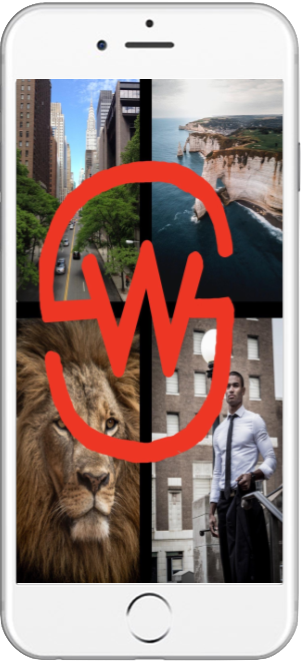
\includegraphics[width = 0.3\textwidth]{imgs/sw_splash.png}

	\caption{SmartWallpapers logo screen}

\end{wrapfigure}

SmartWallpapers will be a lifestyle app that aims to help the users to stay positive in their lives by changing the phone’s wallpaper tailored to user’s preference and giving the possibility to add a motivational quote on top of the wallpaper. It will use Google’s machine learning services in the background in order to figure out the content of a image liked by the user so that in the future it will display on the home screen images with similar content (e.g. only nature phtography or cityscape photography). The wallpaper is changed automatically at a predefined time interval chosen by the user (e.g. 30 min). By changing the wallpaper automatically and the possiblity to set motivational quotes (even created by the user) the app gives the user the chance to see new places and stay motivated throughout the day, take his/her away from the daily routine and daydream about beautiful places from around the world.


\section{Research Developments }

	In this section I will discuss the current and future types of \textit{User Interfaces}. In order to talk about the future it is often good to know what has happened in the past, in our case, the past of \textit{User Interfaces}. In the early days of computing, around 1940s, computers used punched cards (paper cards having perforated holes) to read data and to execute programs (set of instructions stored on these punched cards). In this stage, there is no actual \textit{User Interface}, the computer just reads input and outputs the result of computation. One example of a program that can be stored on a set of punched cards is a basic algorithm used to fire a torpedo at a moving target (submarines in World War 2 used a program of this kind). However, this type of computing is pretty limited in the sense that there is no interaction between the human and the computer, there is no memory and it takes time to obtain valuable results. \\

	\indent 
	The first type of user interface for a computer was developed around 1950s for interfacing with computers over teletypes machines and became popular from 1965-1980  . At that time, roughly 1965-1980, computers were more than basic computation devices (i.e. they resembled modern day computers). This type of user interface allowed the user to interact with the computer by issuing commands, that's why it is known as \textit{Command Line User Interface (CLI)}. It is known that this type of user interface is not for non-technical people and computers having only this type of interface would have not been succesfull for the general-purpose computer market. However, this type of interface is widely used among computer specialists even at this time since it provides a faster way to interact with the computer than Graphical User Interface (GUI) (to be discussed later). Modern operating systems have programs that provide CLI like Command Prompt (Windows) and Terminal (macOS/Linux). The author is using CLI and a text editor program running within the terminal (i.e. VIM) for writing this document. \\

	\indent
	The next stage for user interfaces is represented by GUIs which was developed by \textit{Standford Research Insitute} between 1960-1966. This user interface allows  users to interact with the computer in a more friendly way than the previous one - CLI. Software programs have GUIs (i.e. windows with buttons and text) through which the user can  solve certain tasks. This type of user interface was popularized to the mass-market by Apple in their's Lisa(1983) and Macintosh(1984) computers.\\

	\indent
	The advances in speech recognition and natural language processing pave the way to  a new type of user interface, namely, \textit{Voice User Interface} (VUIs). This type of user interface allows the user to issue voice commands in order to solve certain tasks (e.g. "Alexa, set an alarm for 30 minutes"). There are various types of VUIs on the market right now, but most important are: Siri, Google Assistant and Alexa. Sometimes to use a GUI is not feasible, for example when driving, having a monitor and keyboard in a certain room is not practical or for users with disabilities. The  VUIs allow user to focus his/her attention to some other task while interacting with a computer system. However, there are some challenges for VUIs like no clear distinction on what the system can do (might lead to frustration sometimes for the users). In order to start using a VUIs interface the user needs to first calibrate the system with his voice. There is still a long way until VUIs are adopted by the mass-market.\\

	\indent
	SmartWallpapers will use a GUI for the moment but in the future there is the possibility to integrate it with the personal assistants like Siri(iOS) or Google Assistant(Android) that take voice commands to perform tasks. Now, because we are talking about the User Interface Design (UID) of a mobile app and not of a desktop application, special care needs to be taken. Apple(2018) and Google(2018) have published for their platforms guidelines on how to design the user interface, below the author will present the most relevant guidelines for SmartWallpapers.

\subsection{App Organization}
	There are four major ways of presenting the content of the app to users: 
		\begin{itemize}
			
			\item scrolling pages and cards - for apps that provide content in categories (e.g. photo gallery)

			\item bars and drawers -  for apps with multiple sections of content (e.g. Facebook: news feed, requests, messages etc.)

			\item tree hierarchy - for apps with large number of features organized in categories which allow the user to drill down (e.g. Spotify: classic -> Andre Rieu -> album X -> songs)

			\item content-driven - ideal for games where the developers want to provide a specific experience 

		\end{itemize}

	SmartWallpapers will use the \textit{scrolling pages and cards} organization style due to the fact that it needs to present the content (photos) in categories (e.g. nature, night sky, cityscape etc.).

	\subsection{Making Choices}
	Since the user of a mobile device might  on moving when using the device it is not practical to type, thus if possible is better to avoid asking the user to type anything. Both platforms (Android and iOS) provide widgets for making choices without the need for keyboard input. One example of such a widget is a picker which allows users to "pick" a date or set a timer, in our case, the user will be able to "pick" the change wallpaper interval.

	\subsection{Shortcuts}
	Gestures can really make the difference and are a way to speed-up things for advanced users. However, they need to be intuitive, easy to discover and easy to use. There are a set of standard gestures like: double-tap to zoom, tap and hold to copy, shake to undo or swipe to delete. For our app, the use can swipe left or right to express his/her preference regarding a certain photo. One important aspect of a system is to provide feedback (Norman, 2013) and especially for gestures.


	\subsection{Onboard users quickly}
	The first time the user encounters an app is decisive; if the user can understand the benefits and how to use it then the user will keep the app.
Some features must be introduced to the user via a tutorial, this tutorial should contain also the reasons to keep the app.

	There are 5 methodologies to onboard users:
	
	\begin{itemize}
	
		\item benefits-oriented -> show some images (max 3 recommended) with the benefits of the app at first launch

		\item function-oriented -> show some images (max 3 recommended) with the basic features of the app

		\item progresive        -> the features are explained when the user encounters the triggers (e.g. buttons, images etc.)

		\item hybrid            -> combine benefits-oriented / function-oriented with progresive onboarding 
		
		\item video -> create a short presentation video (less than 1 min) 

	\end{itemize}
	
	To sum it up, apart from the functionalities the app provides having a good design plays a decisive role in app aquisition and app retention.

\section{Sector}
	
	In order to better understand the market and to develop an useful app a market analysis was required. In the following lines there is going to be presented similar apps to SmartWallpapers.

\subsection{Google Wallpapers}
		
		\begin{wrapfigure}{R}{0.3\textwidth}
	
			\centering
			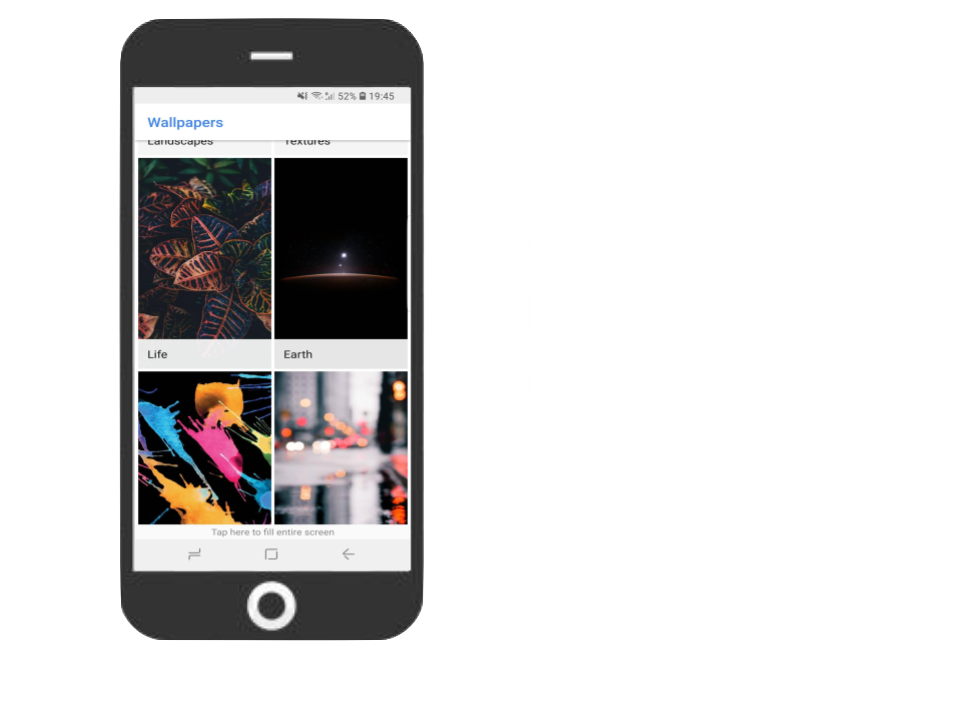
\includegraphics[width=0.6\textwidth]{imgs/Google_Wallpapers.png}
			\caption*{Google Wallpapers}

		\end{wrapfigure}

		When it comes to applications developed by Google we as users always expect state of the art, some successful apps from them are \textit{Google Translate}, \textit{PhotoScan} or \textit{Google Photos}. However, \textit{Google Wallpapers} is pretty simple in my opinion. The range of wallpapers that it provides is quite small, you can select your wallpaper to be changed daily (but you can't change it every 2h if you choose to). Overall, it is a useful application but pretty limited in my opinon.


		\subsection{Wallpaper Changer}
		What \textit{Google Wallpapers} lacks, the feature to set the interval at which the wallpaper should be changed, this application provides.
Also, it gives you the possibility to select a folder from system explorer with the image sources that are going to be used to change the wallpaper. There are other small features that this app provides, however the UI design is poor, the "Set Wallpaper"  feature does not work on my device and there is no tutorial for the app (is hard to learn how to use it).\\

		\indent
		To address the above mentioned drawbacks of the apps in this sector and to bring something new to the market \textit{SmartWallpapers} is going to be developed.
		What makes our app different from what is already on the market?

		\begin{itemize}
			\item the automatic wallpaper changing without the need for the user to provide the photos (using his/her photography preferences)

			\item the possibility to set the wallpaper changing inteval (compared to \textit{Google Wallpapers})
			
			\item a large set of photos to choose from, changed each 2-3 days from unsplash.com

			\item the possibility to set a quote on top of the wallpaper

			\item the possibility to search photos based on location or by input query

		\end{itemize}

\newpage

\section{Personas \& User Requirements}

\subsection{Persona 1}

\begin{wrapfigure}{R}{0.4\textwidth}
		
	\centering
	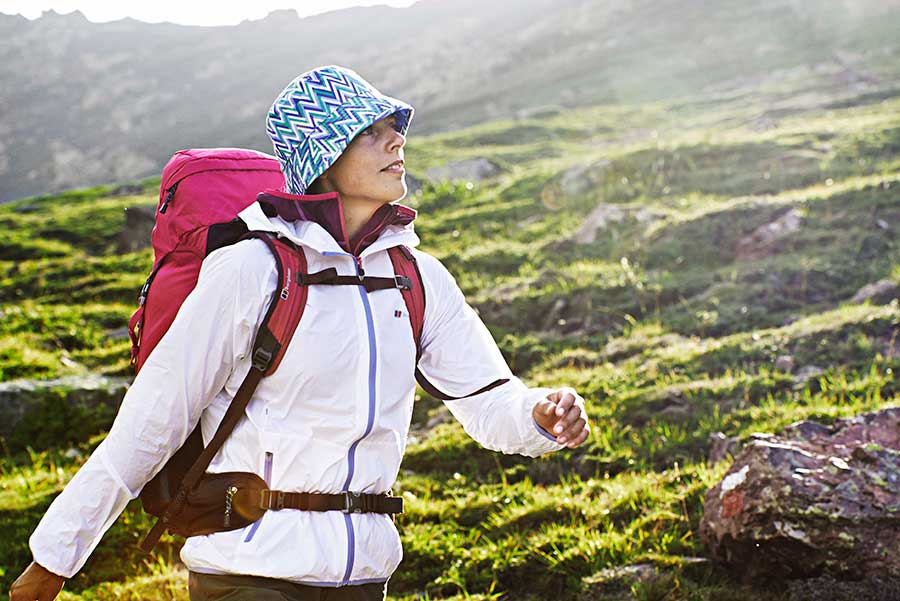
\includegraphics[width = 0.5\textwidth]{imgs/Lisa.jpg}
	\caption*{Persona 1: Lisa - traveller}

\end{wrapfigure}

\noindent
Name: Lisa \\
Age: 40 \\
Occupation: Travelling Agent \\
Location: London, UK \\
Tech Level: Moderate \\
User Requirement: 
	\begin{itemize}
		\item  app easy to use
		\item  find location of a photo
		\item a lot of content
		\item  ability to share photo 
	\end{itemize}

 After receiving a bachelor degree in \textit{English Language and Literature} Lisa has taught English in several different countries from Asia and Middle East. While she was there she travelled around and saw the world. Based on her travelling experience she has been given a position as travelling sales agent at a company based in London. She decided that was time to go home and accepted the position. Although being home is good she doesn't have that much free time to travel around as in the past so whenever she has a free weekend she wants to make the most of it and go to an amazing location.

\subsection{Persona 2}

\begin{wrapfigure}{R}{0.4\textwidth}
		
	\centering
	
\includegraphics[width = 0.5\textwidth]{imgs/Alan.jpg}
	\caption*{Persona 2: Allan - businessman}


\end{wrapfigure}

\noindent
Name: Allan\\
Age: 35\\
Occupation: Project Manager\\
Location: New York, USA\\
Tech Level: Expert\\
User Requirement:
	\begin{itemize}
		\item ability to customize app and use shortcuts
		\item possibility to add motivational quote on home screen
		\item ability to share photo
	\end{itemize}

	Allan is a Project Manager for a top tech IT company in Manhattan (New York) and he works 996 (each day from 9am to 9pm and 6 hours on a Sunday). He is an achievingtype of person and has dedicated his whole life to career. Having such a busy program, sometimes he needs some extra motivation or to see a new place even on his smartphone screen. Nonetheless, there is no time for daydreaming and browsing the internet to look for motivational quotes or photography.

\subsection{Persona 3}


\begin{wrapfigure}{R}{0.3\textwidth}
		
	\centering
	
\includegraphics[width = 0.4\textwidth]{imgs/Patrick.jpg}
	\caption*{Persona 3: Patrick - young professional}


\end{wrapfigure}

\noindent
Name: Patrick\\
Age: 27\\
Occupation: Junior Software Engineer\\
Location: Dubai, United Arab Emirates\\
Tech Level: Expert\\
User Requirement:
	\begin{itemize}
		\item lots of content
		\item always new photography
		\item location based photography
	\end{itemize}

Patrick has just moved to Dubai to work for a new IT startup with great potential. During his childhood he travelled a lot with his family but they did not afford to visit Middle East so this job opportunity seemed appealing to him. Because he works for a startup he doesn't have that many colleagues, moreover, he doesn't speak Arabic so making new friends outside of work seems hard. He decided to visit the Middle East as much as possible while he is there. An application that could show him nearby sights seems interesting to him.

\subsection{Persona 4}

\begin{wrapfigure}{R}{0.3\textwidth}
	
	\centering
	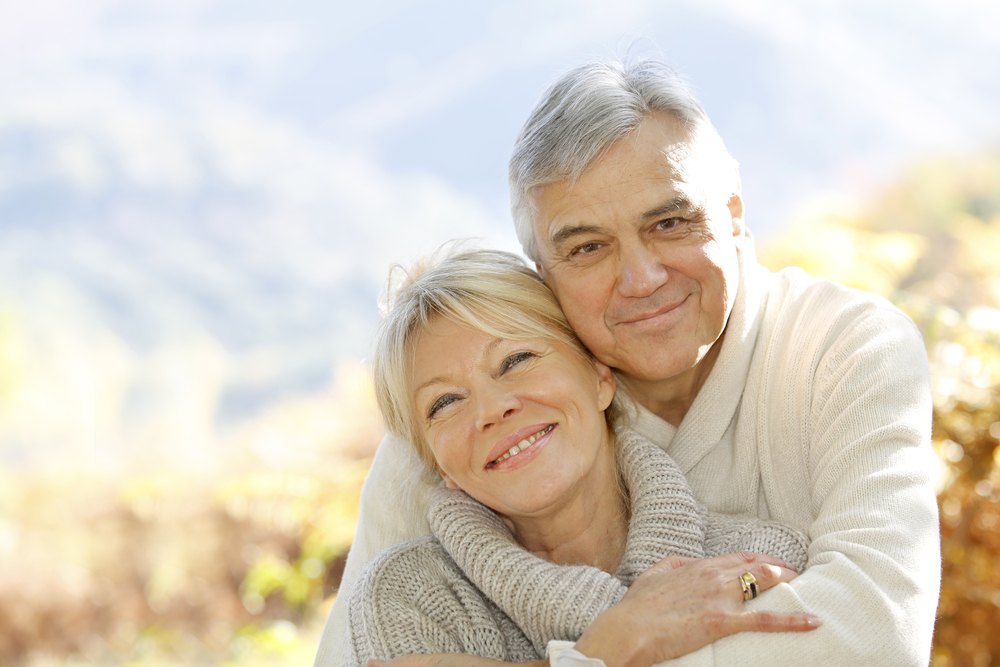
\includegraphics[width = 0.4\textwidth]{imgs/Anne.jpg}
	\caption*{Persona 4: Anne - retired diplomat}

\end{wrapfigure}

\noindent
Name: Anne\\
Age:  62\\
Occupation: Retired Diplomat\\
Location: Washington, DC\\
Tech Level: Basic\\
User Requirement:
	\begin{itemize}
		\item easy to use 
		\item help after a mistake has been made when using the app 
		\item possibility to see photos from visited places
	\end{itemize}

	Anne and her husband have been working for different USA Embassies in different corners of the world. Now they enjoy their retirenment and like to be at home in DC.However, they enjoy seeing fresh photography from the places where they lived and are interested how the politic situation is evolving at home and abroad. They are amazed how the technology is making things possible and are open to learn how to use it.

\section{Designs}
//multiple possibilities not good - i don't think it refers to gestures (e.g. tinder) \\

//feedback for each action \\

//knowing what to do: heart with green and cross with red (?)\\

//give possibility to go back to last photo in case wants to revise his decision (but only to the last one, he can't go all the way back)\\

//have actions that match users intentions (e.g.: Download a photo, beside being able to use it as wallpaper)\\


	In the  following lines I am going to present and discuss the designs for a prototype version of this app.

\subsection{Photo categories interface}
\begin{wrapfigure}{R}{0.3\textwidth}

	\centering
	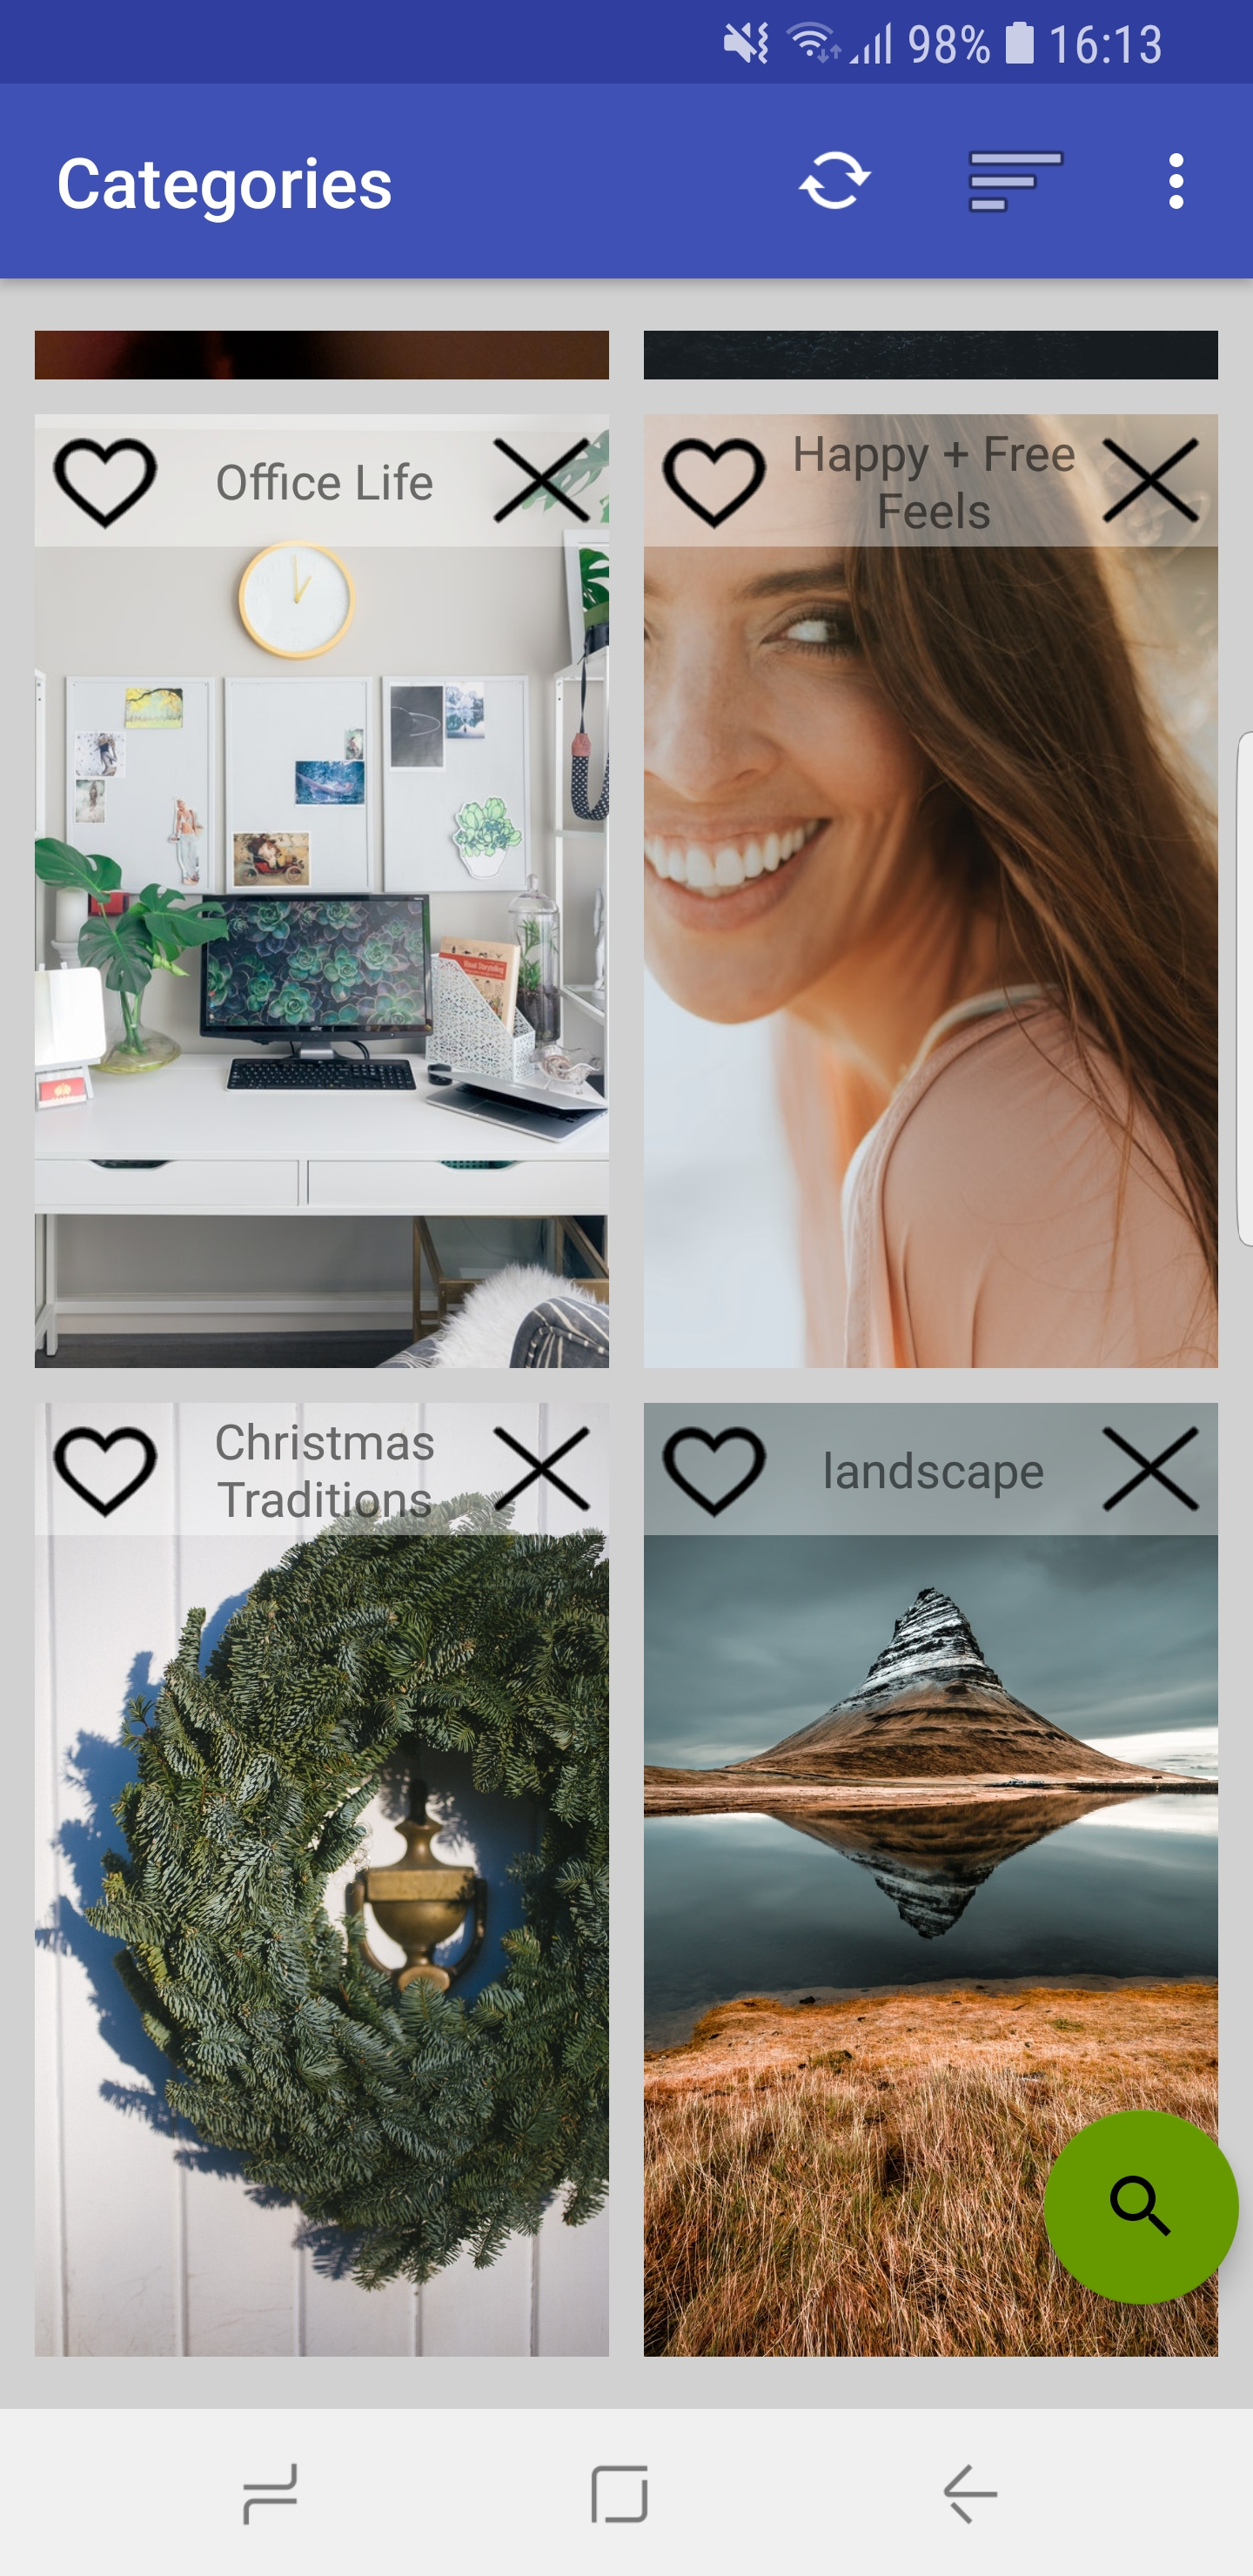
\includegraphics[width = 0.3\textwidth]{imgs/Categories.jpg}
	\caption*{Fig 2: Photos organized in categories (albums)}

\end{wrapfigure}
	In order to provide  users with different types of photography and a large set of photos, SmartWallpapers uses an online provider, namely \textit{unsplash.com} .
This is ideal for Lisa (Persona 1) and Patrick (Persona 3) who want a lot of content to be provided by the app .From the 4 app organization methodologies presented in the \textit{Research Developments} section, SmartWallpapers uses \textit{scrolling pages and cards}. Each type of photography is organized in categories; the categories change each 2-3 days. As it can be seen in the screenshot to the right of text, there is a category dedicated to\textit{Christmas}, since it is close. \\

	In this screen the user has multiple possibilites to interact with the app, we're going to present the most important ones. For each type of category there are 2 types of possible actions: like (heart button) or dislike (cross button). If the user likes a category then all the photos from within will be queued to be displayed on the screen. After liking it, the category (or album) disappears from this screen. The user can also choose to enter in a category by a single tap on it and then like/dislike indivitual photos (see figure ~\ref{fig:transition}). Before entering a category the scroll position is saved.

	%going back from a category save scroll position

\begin{figure}
\centering
\begin{subfigure}{.5\textwidth}
  \centering
  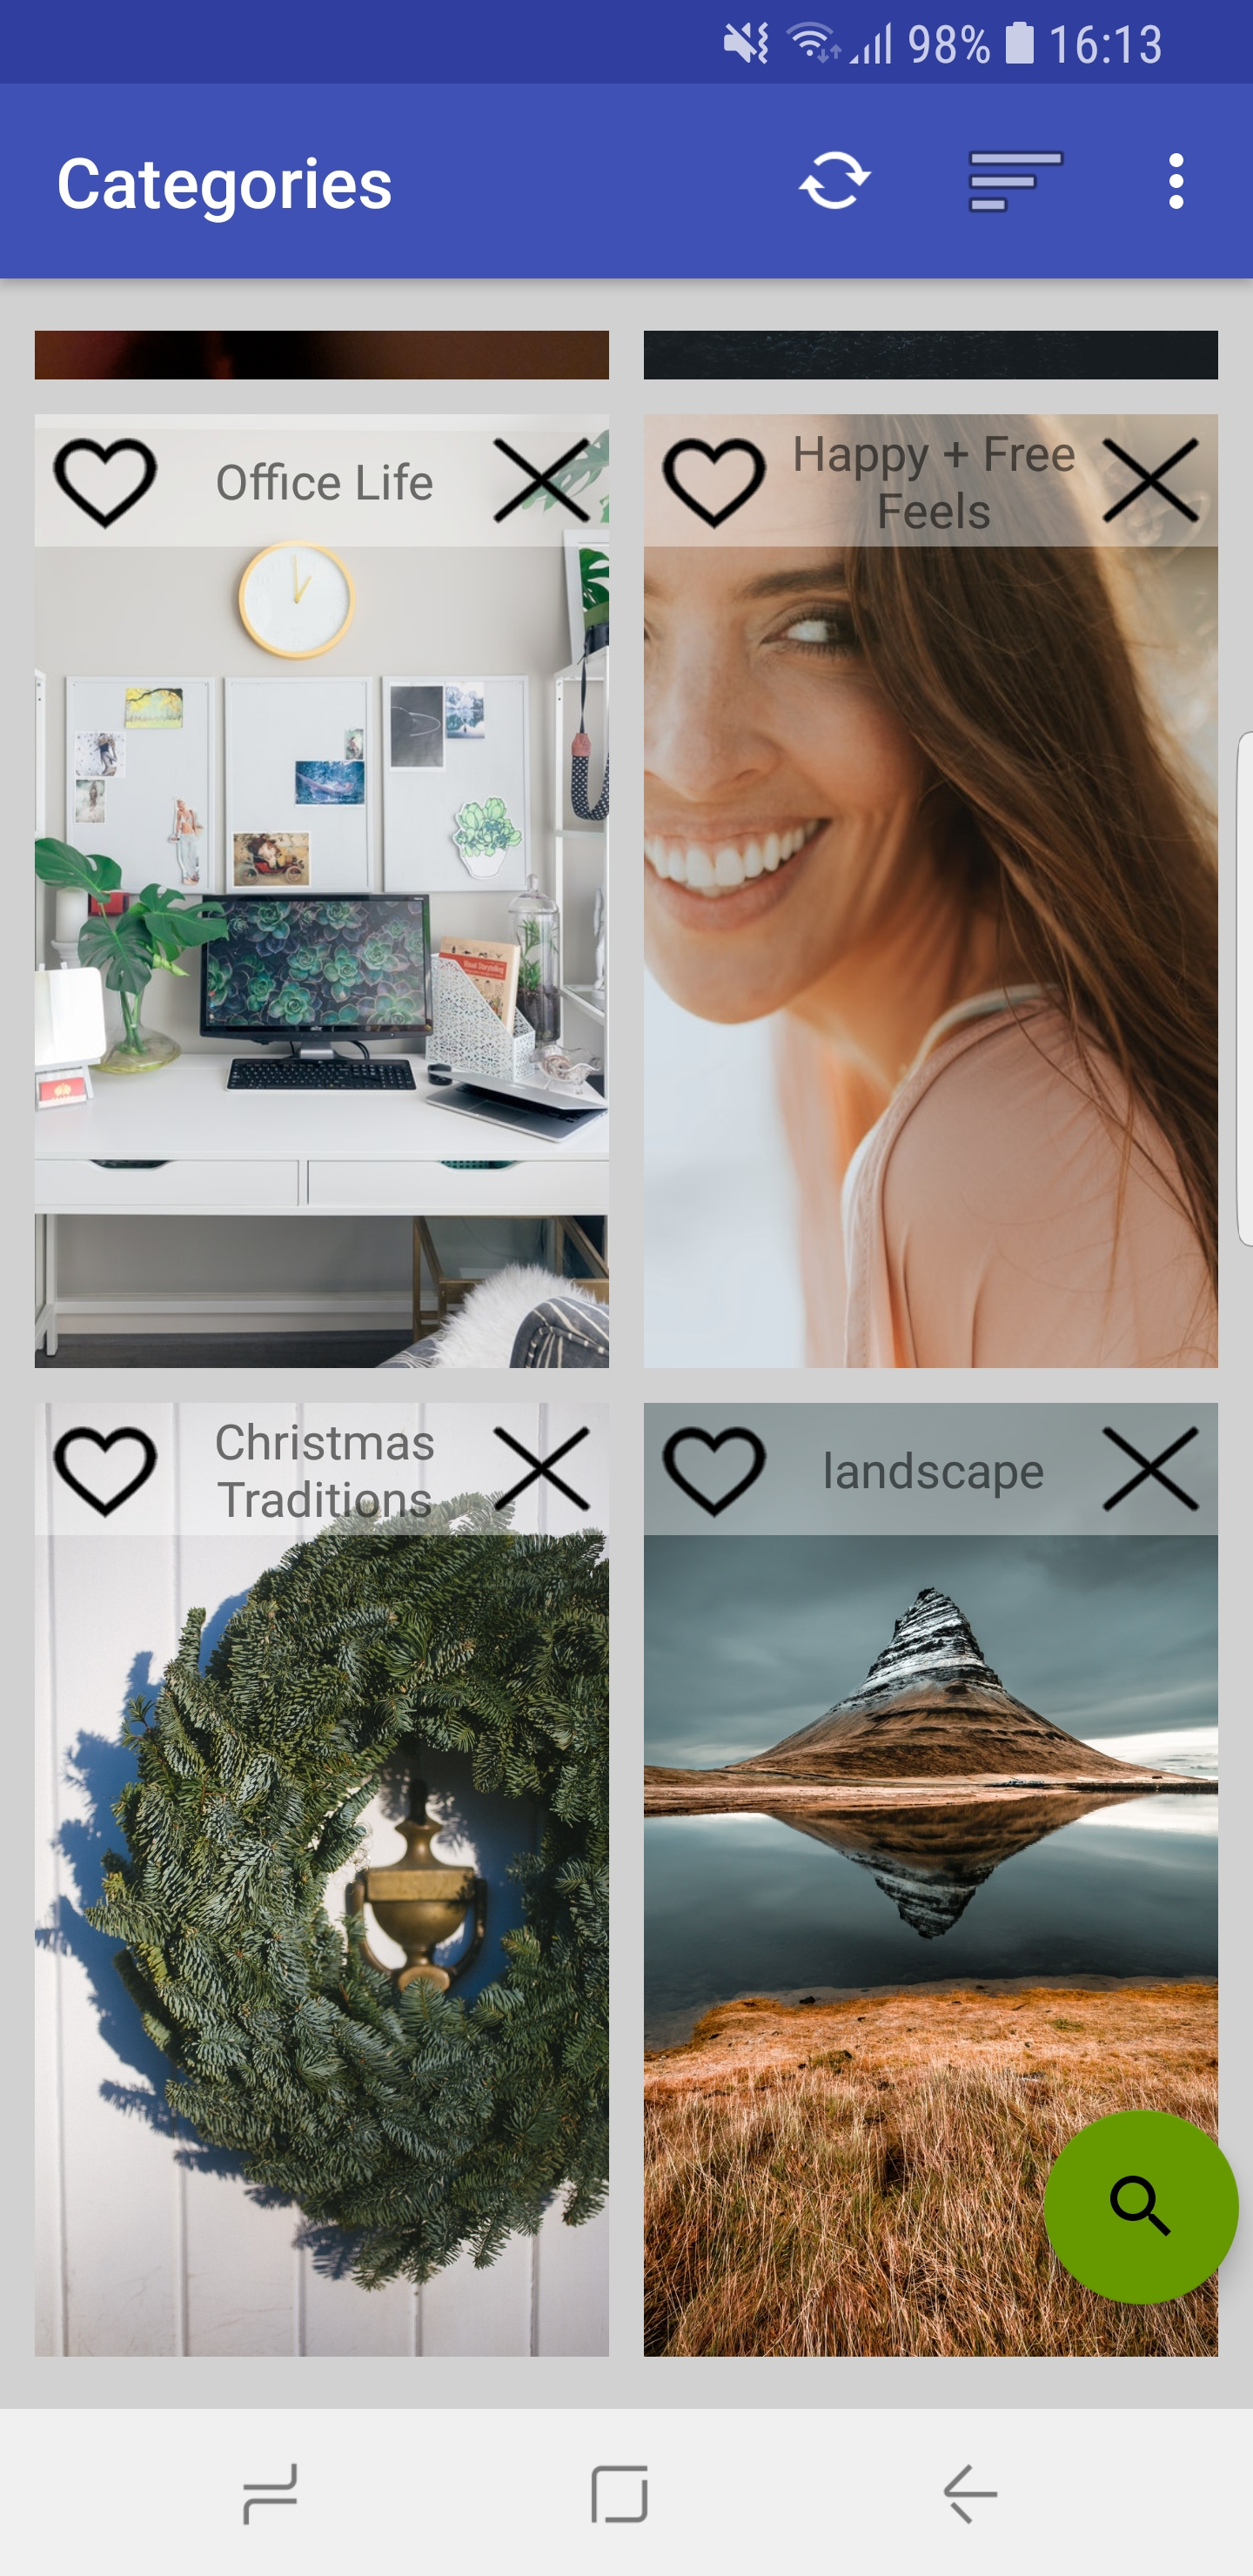
\includegraphics[width=.45\linewidth]{imgs/Categories.jpg}
  \caption{Categories view}
  \label{fig:sub1}
\end{subfigure}%
\begin{subfigure}{.5\textwidth}
  \centering
  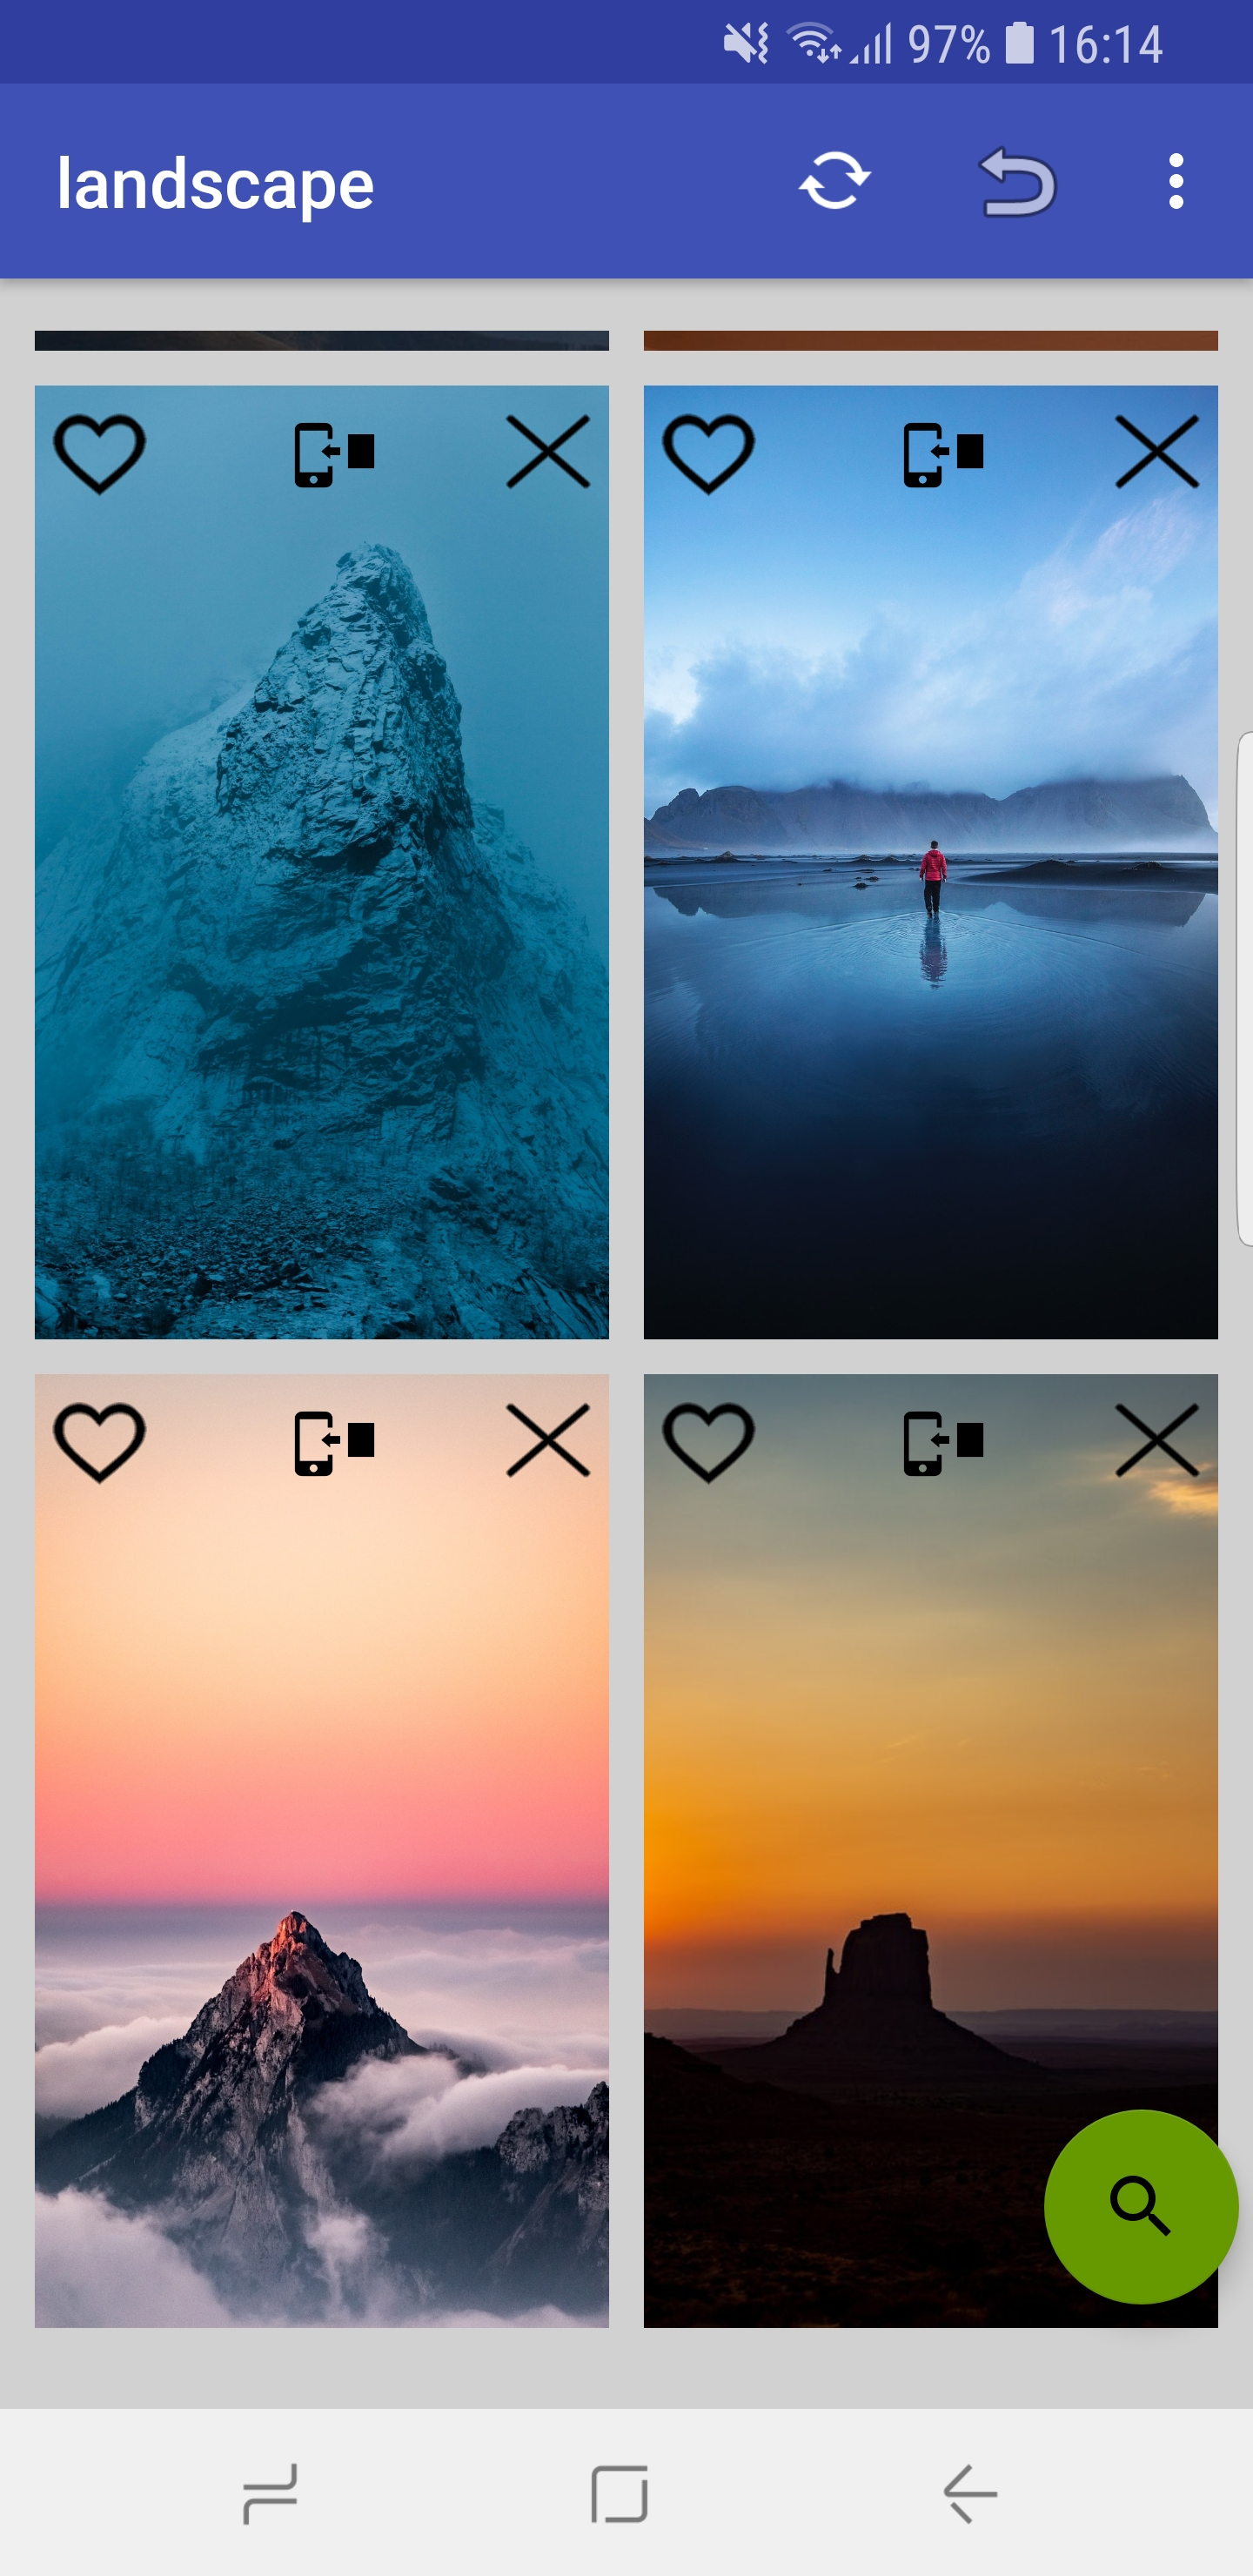
\includegraphics[width=.45\linewidth]{imgs/Inside_category.jpg}
  \caption{View inside "landscape" category}
  \label{fig:sub2}
\end{subfigure}
\caption{Transition from a category to the photos it contains using single tap}
\label{fig:transition}
\end{figure}

\vspace{2cm}

\subsection{Contents of category interface}

\begin{wrapfigure}{R}{0.3\textwidth}
  \centering
  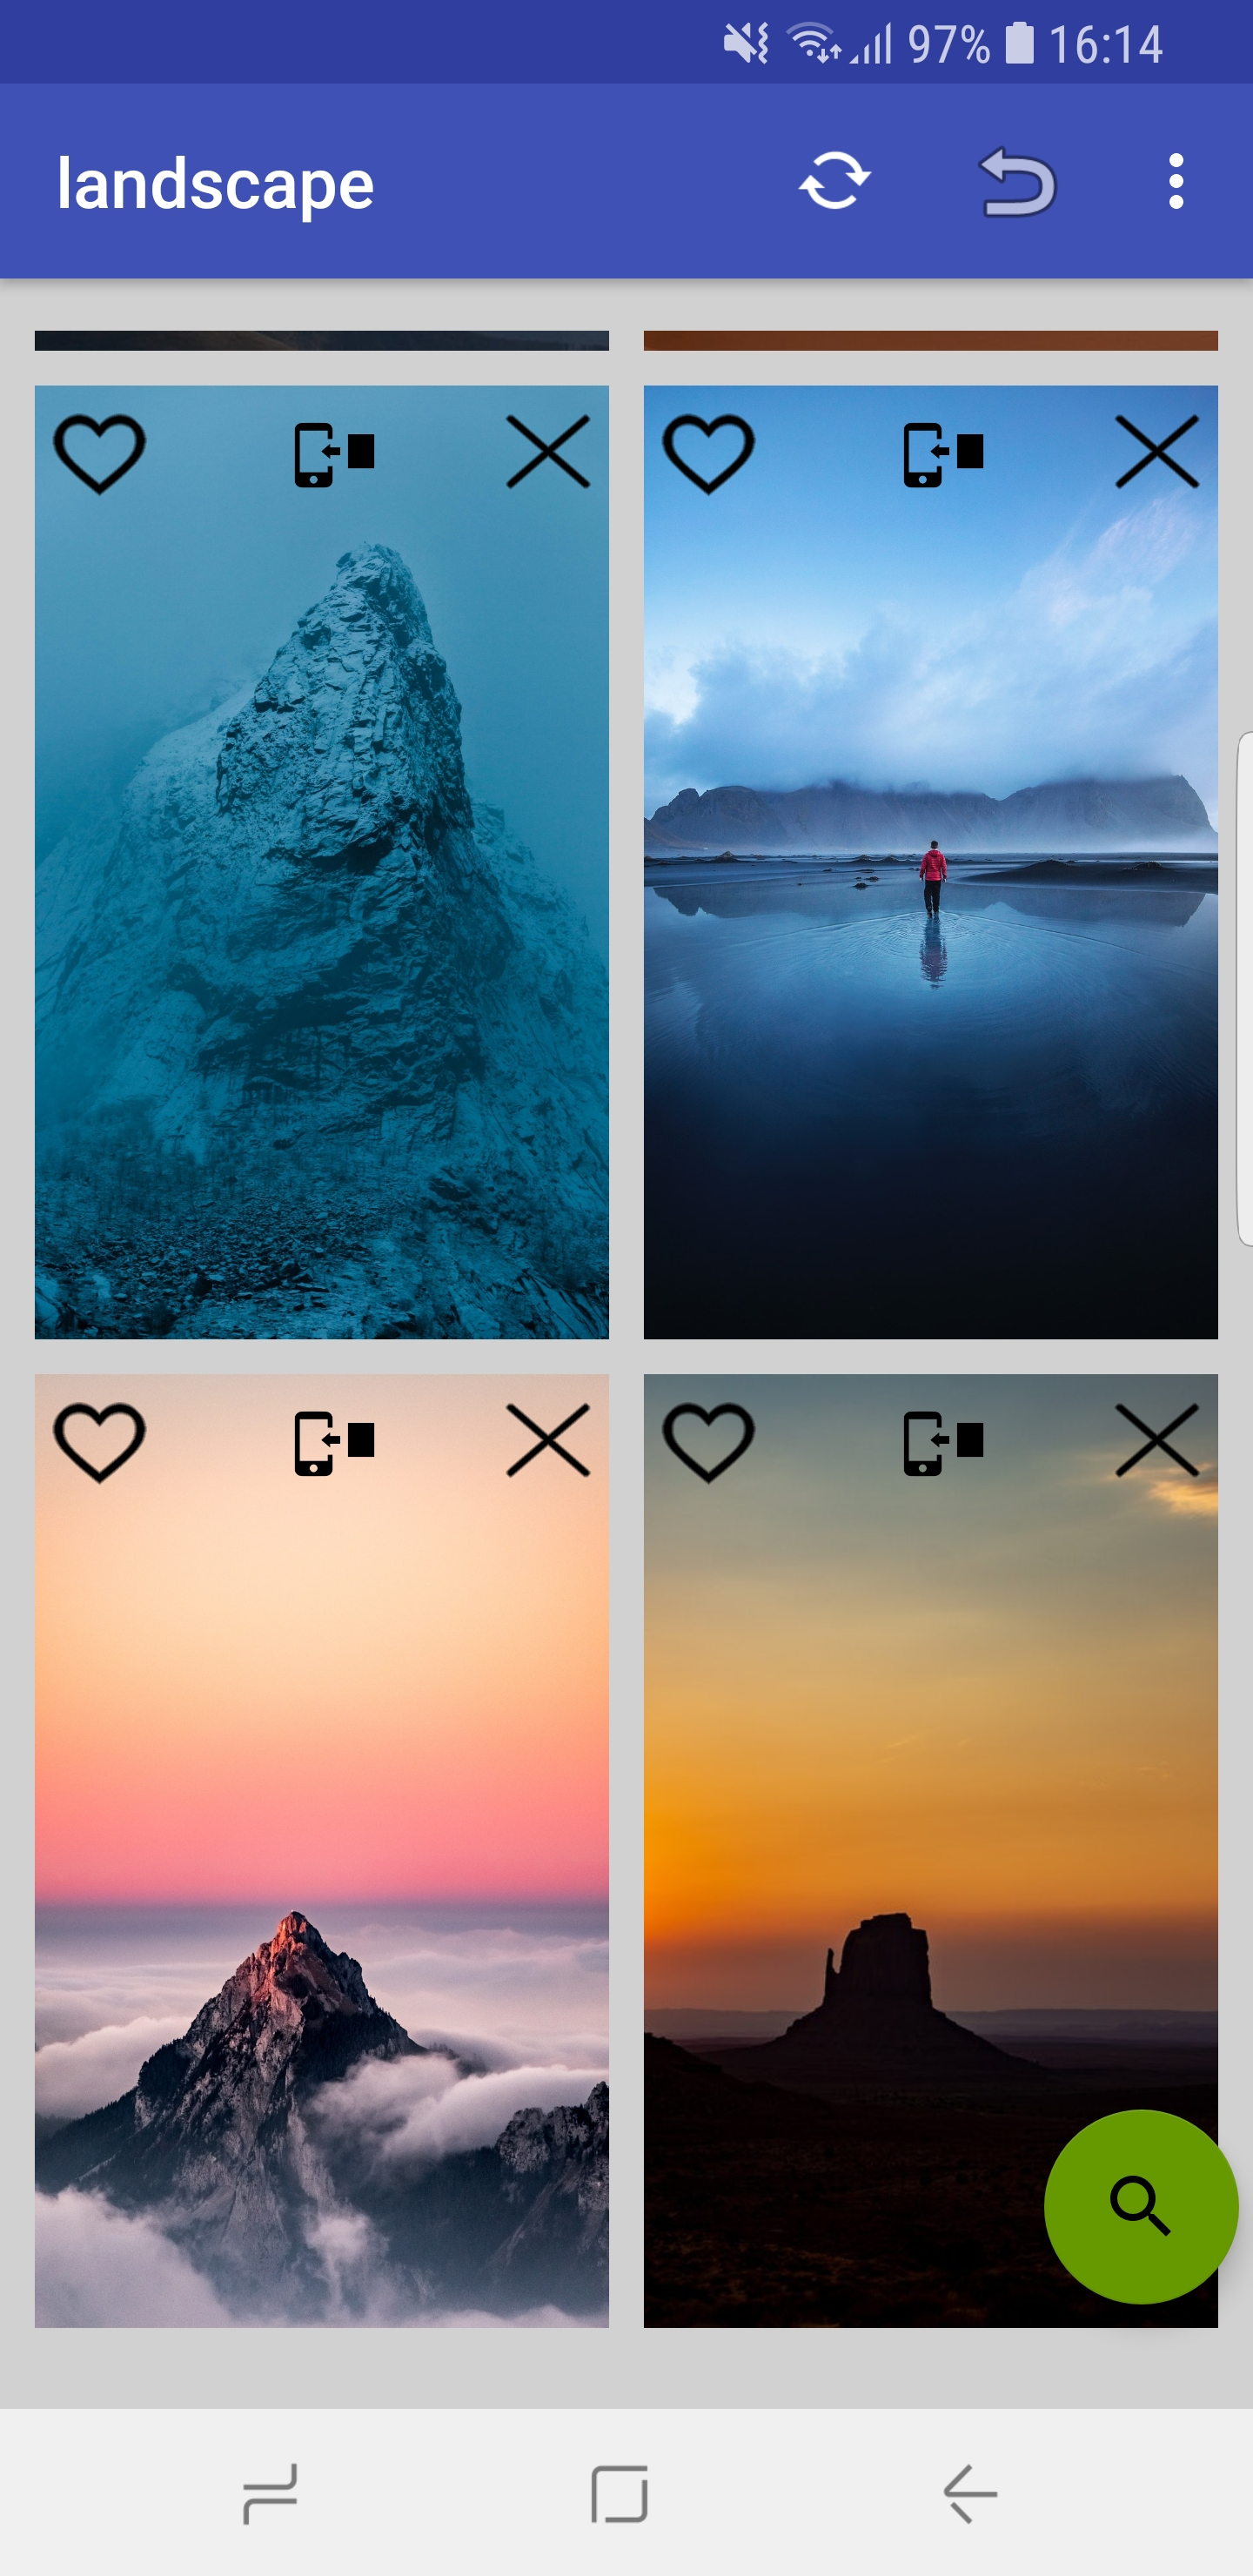
\includegraphics[width=0.3\textwidth]{imgs/Inside_category.jpg}
  \caption{View inside "landscape" category}
\end{wrapfigure}

	As can be seen in the photo from the right, for each photo there are 3 actions that can be performed on it. The actions are (left to right): like (heart icon button), set photo as wallpaper (middle button) and dislike (cross icon button). When tapping like button the photo disappears from the list and is going to be queued for displaying it on the home screen. On tapping dislike button the photo is just taken out of the category. Also, if the user wants it is possible to see a photo in "full-screen" mode by single tapping on it ( Figure ~\ref{fig:fullscreen}). When in full-screen mode, liking/disliking a photo gets the next photo after current one to be dispalyed in full-screen mode. According to Norman(2013) is good not to force the user to perfrom a certain task, thus if the user is undecided simply tapping the photo brings the next one, thus the app is not forcing the user to express his/her preference on the spot. There is also the possibility to close the full-screen mode using the top-right cross button (see Figure~\ref{fig:fullscreen}). I think this interface is easy to use so it suits Lisa (Persona 1) and Anne (Persona 4).\\

\begin{figure}[H]

	\centering
	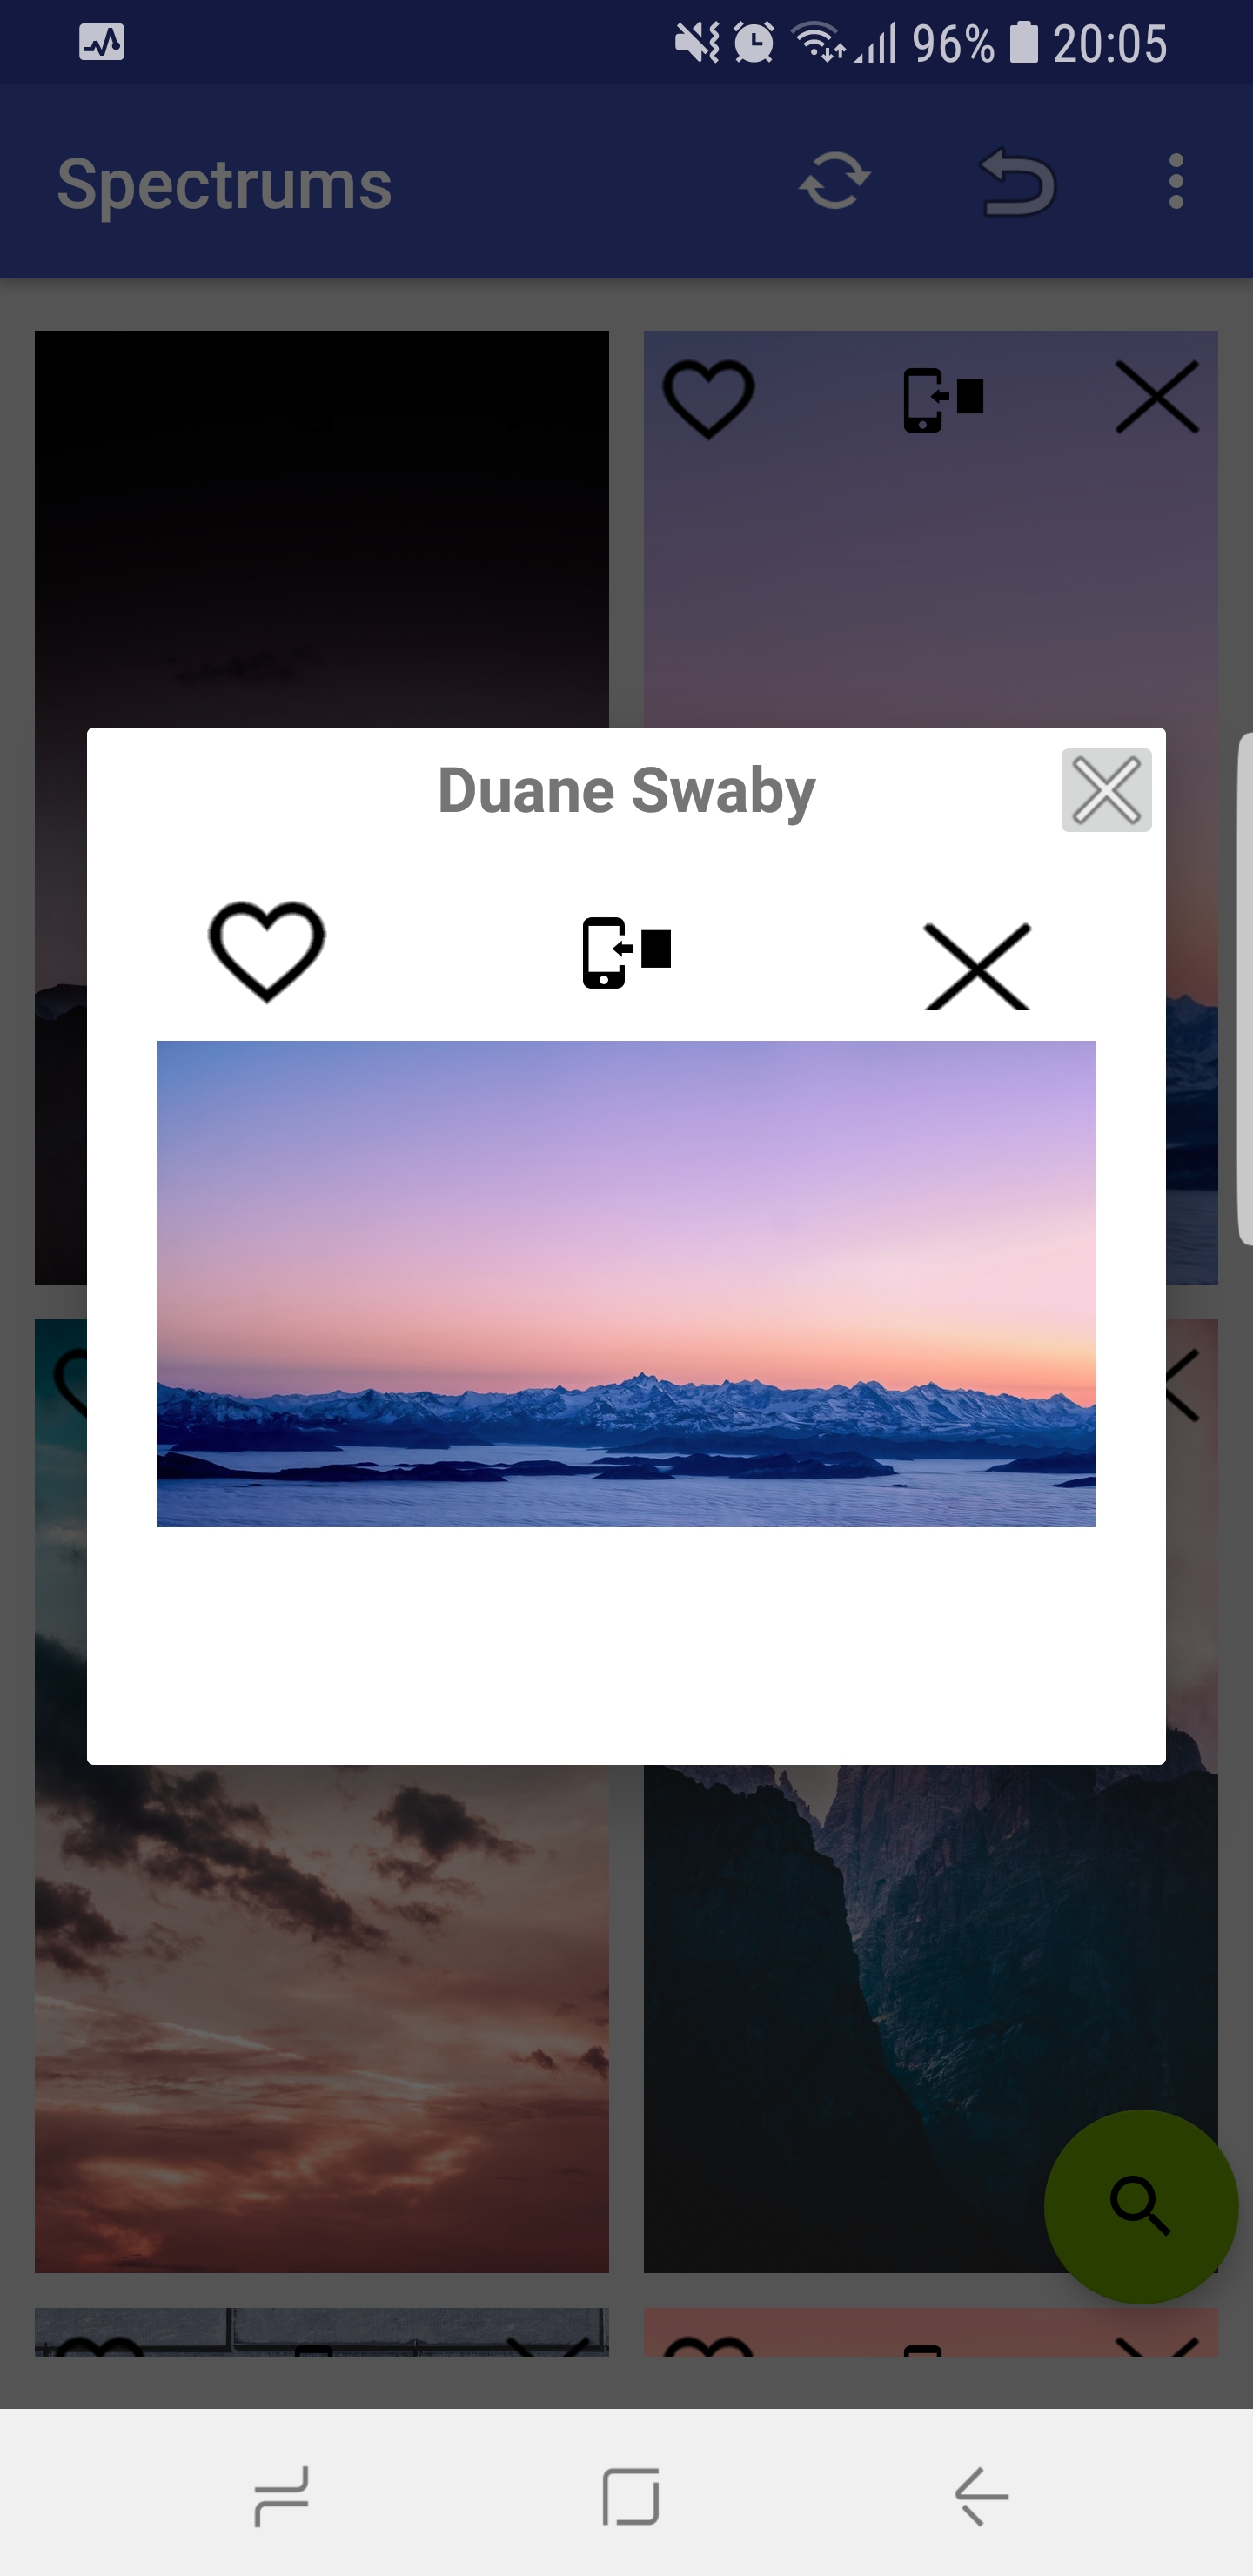
\includegraphics[width = 0.3\textwidth]{imgs/FSPhoto.jpg}
	\caption{View of photo displayed in full-screen mode}
	\label{fig:fullscreen}

\end{figure}

\subsection{Search feature interface}
	The search functionality of prototype-SmartWallpapers allows users to search images based on a query (e.g. "Big Ben", "Eiffel Tower" etc.) or on user's current location (i.e. the country where the user is at a specific time). This is ideal for Patrick (Persona 3) and Anne (Persona 4) who want specific type of photography to be set on their home-screen, places where they have been or where they live.

\begin{figure}[H]
\centering
\begin{subfigure}{.5\textwidth}
  \centering
  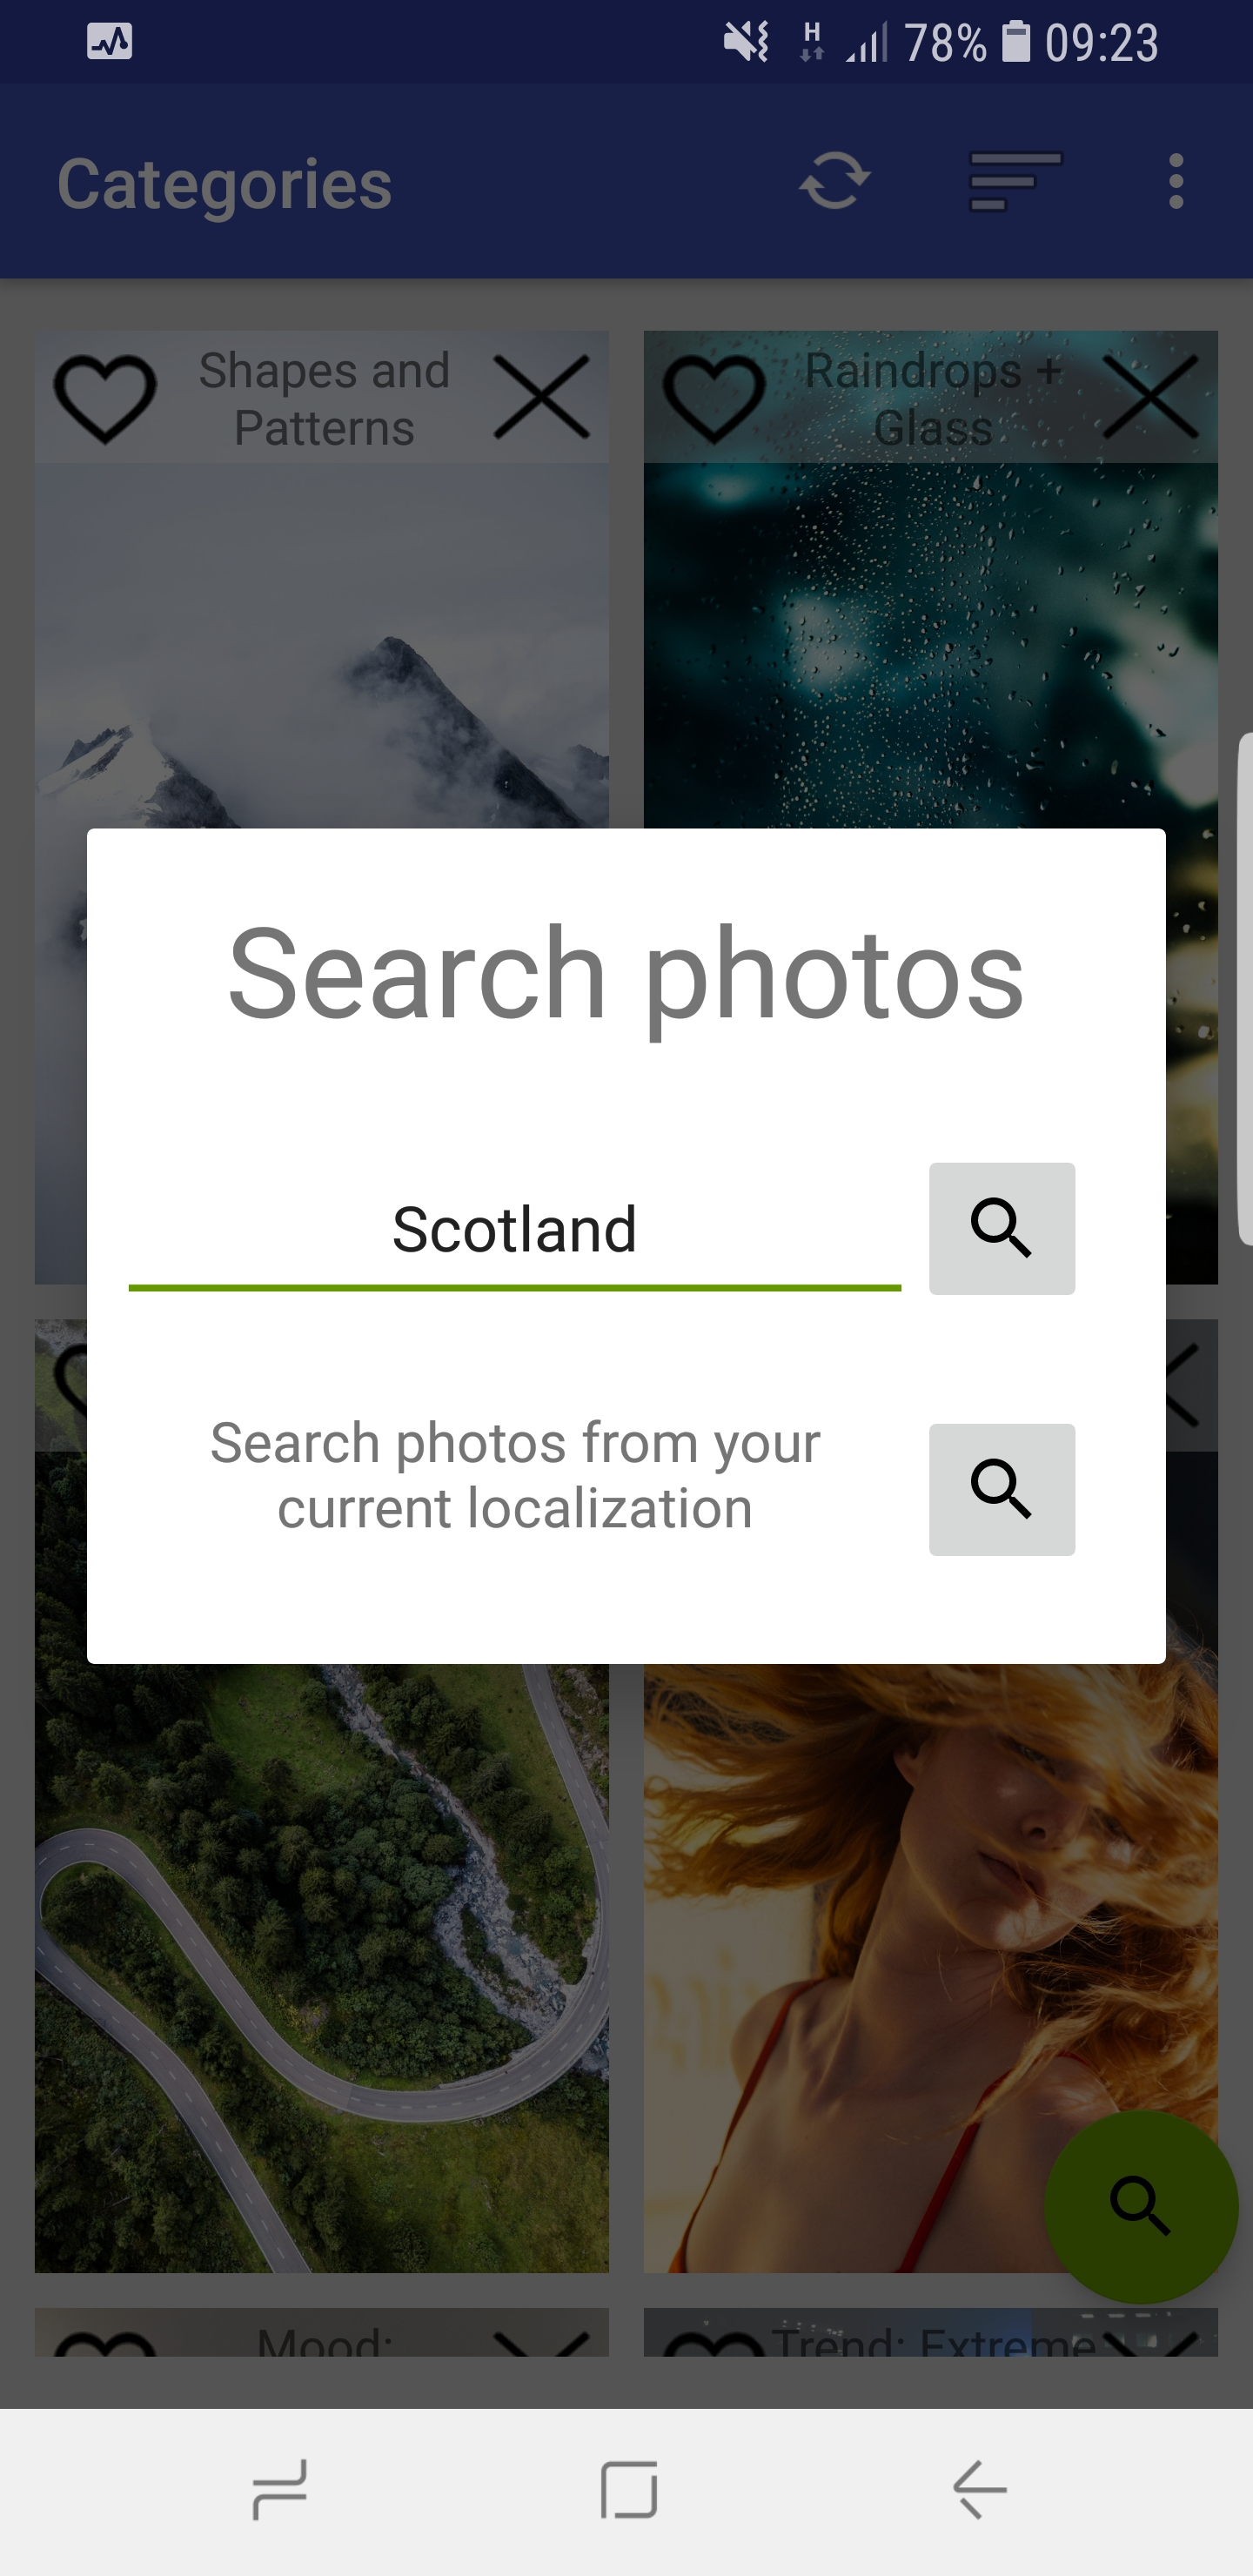
\includegraphics[width=.5\linewidth]{imgs/SearchQuery.jpg}
  \caption{View for performing a search using a query string}
  \label{fig:sub1}
\end{subfigure}
\begin{subfigure}{.55\textwidth}
  \centering
  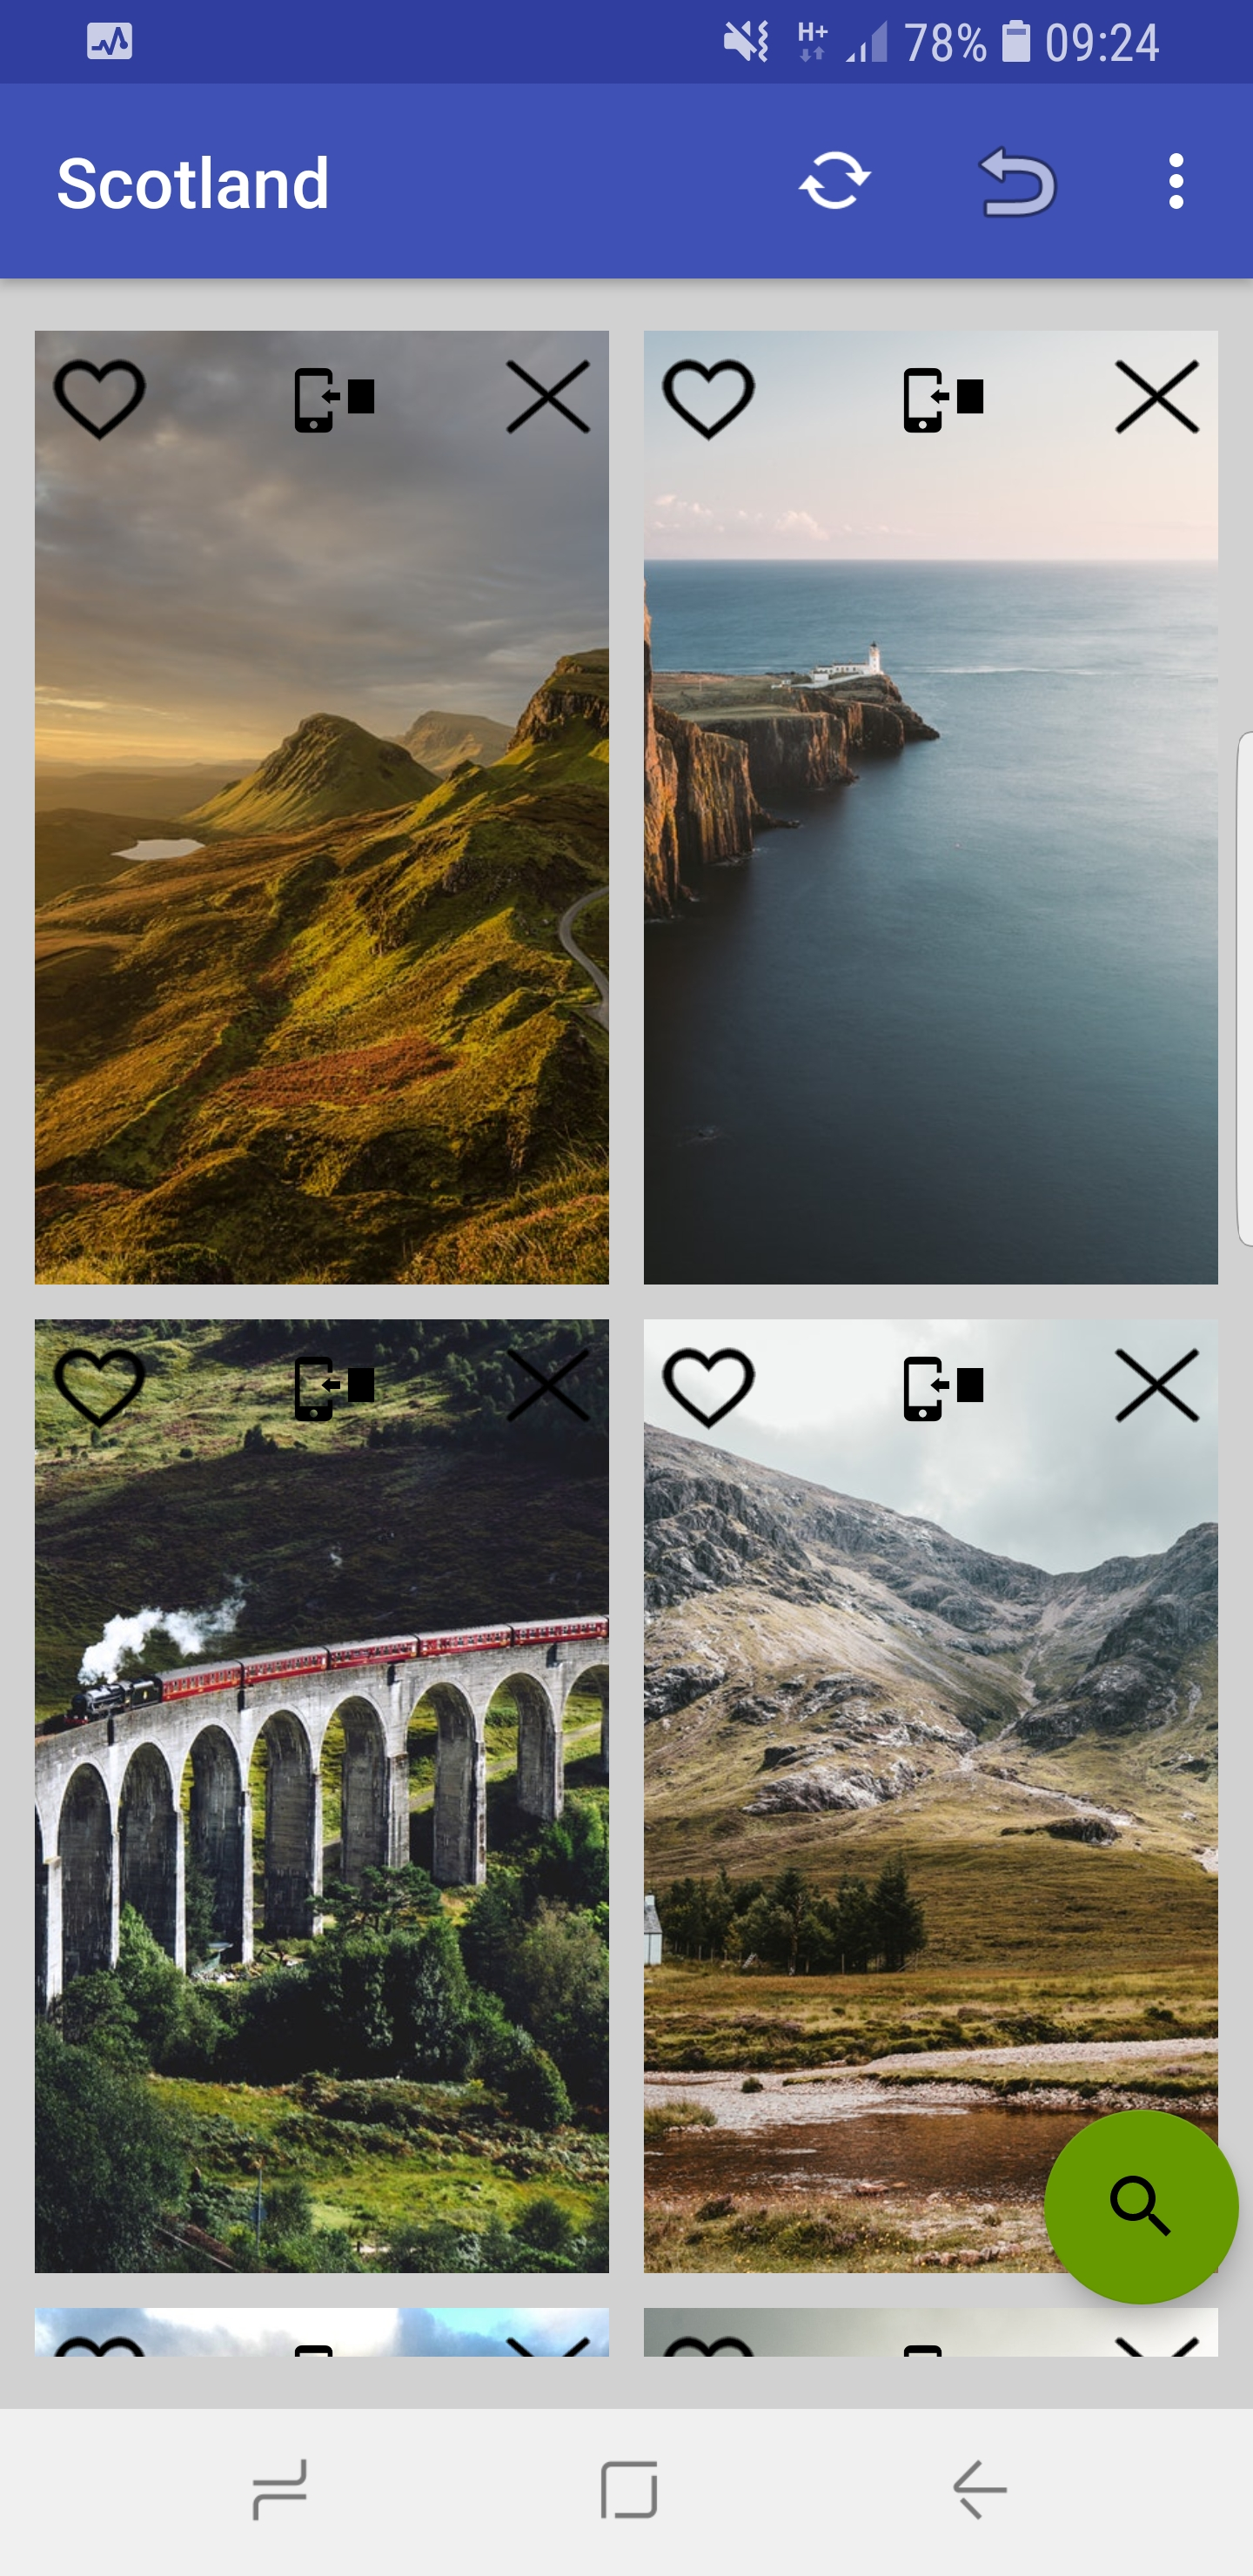
\includegraphics[width=.5\linewidth]{imgs/SearchPerformed.jpg}
  \caption{View displaying the result of the search}
  \label{fig:sub2}
\end{subfigure}
\caption{Performing a search of photos based on query or current location (country)}
\label{fig:transition}
\end{figure}


\subsection{Quotes feature interface}
	For some users it is important to stay motivated and focused on their tasks throughout the day thus being able to see a motivational quote, here and then, when they use their phone is a useful feature. The user is able to pick a quote from a large database of quotes (around 72000) or add his favourite quote and set it on the home-screen. From design perspective, interacting with a quote is the same as with interacting with a photo,  we know that consistency is important. The user  can choose the position (i.e. top, center or bottom), the size of the text (i.e. large, medium or small) and the colour of text (white, black or green)  of the quote that is going to be displayed on the home-screen (see Figure~\ref{fig:setQuote}).  


\begin{figure}[H]

  \centering
  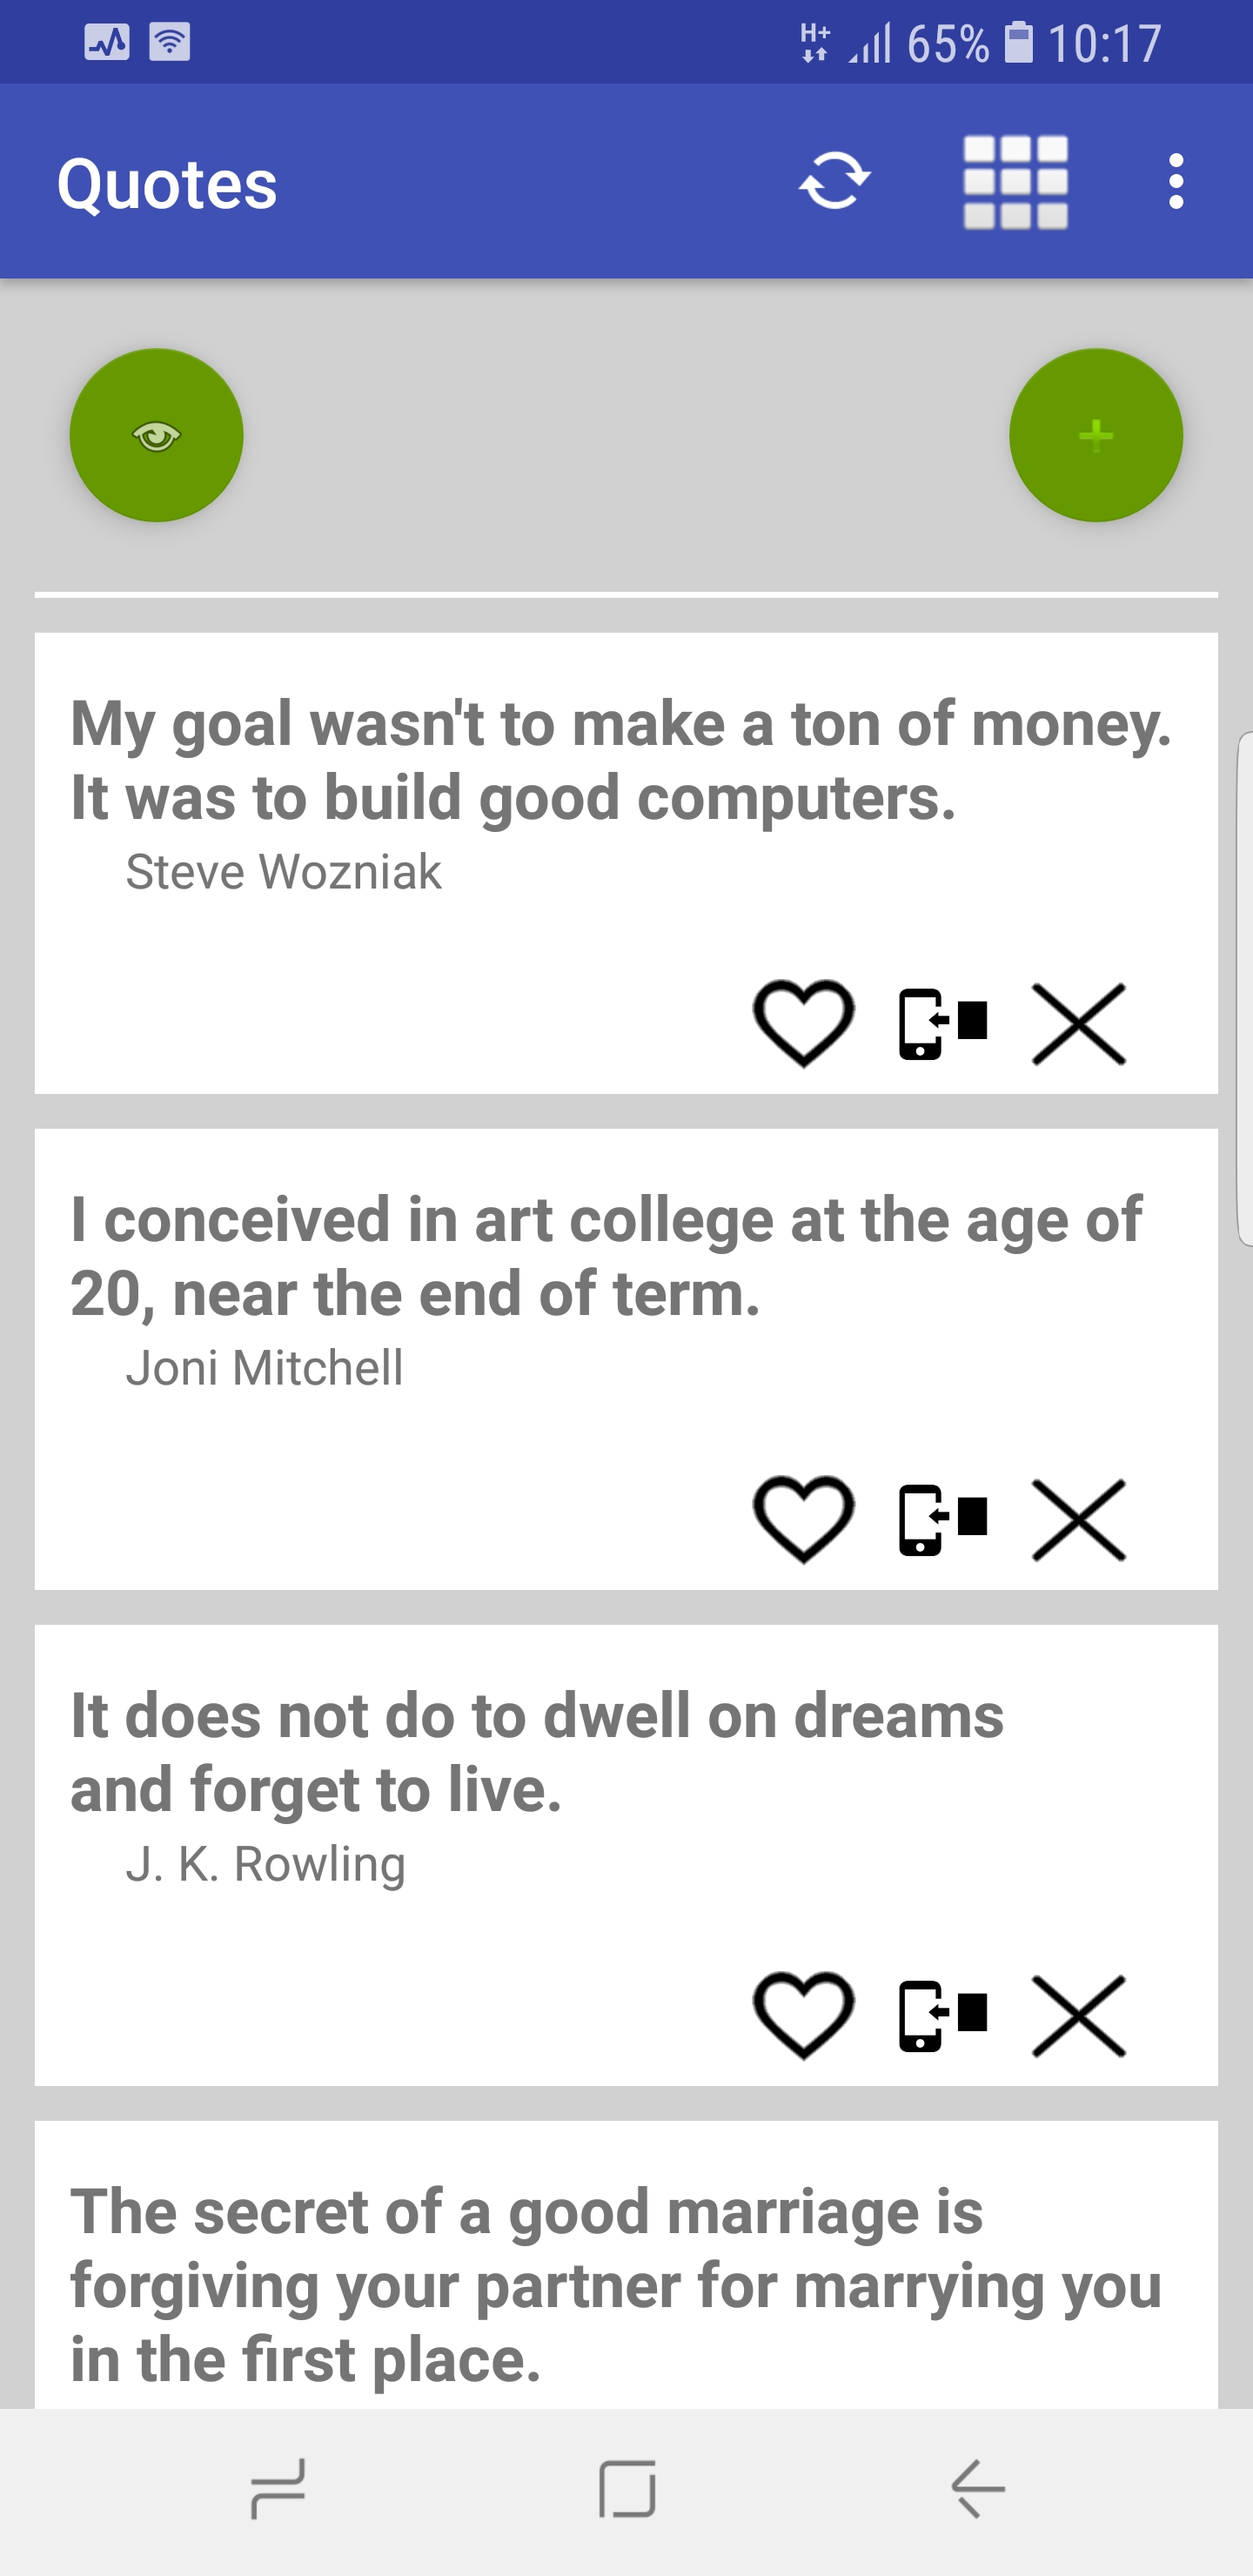
\includegraphics[width=.3\linewidth]{imgs/QuotesList.jpg}
  \caption{View of the quotes}
  \label{fig:quotes}

\end{figure}

\begin{figure}[H]
\centering
\begin{subfigure}{.55\textwidth}  \centering
  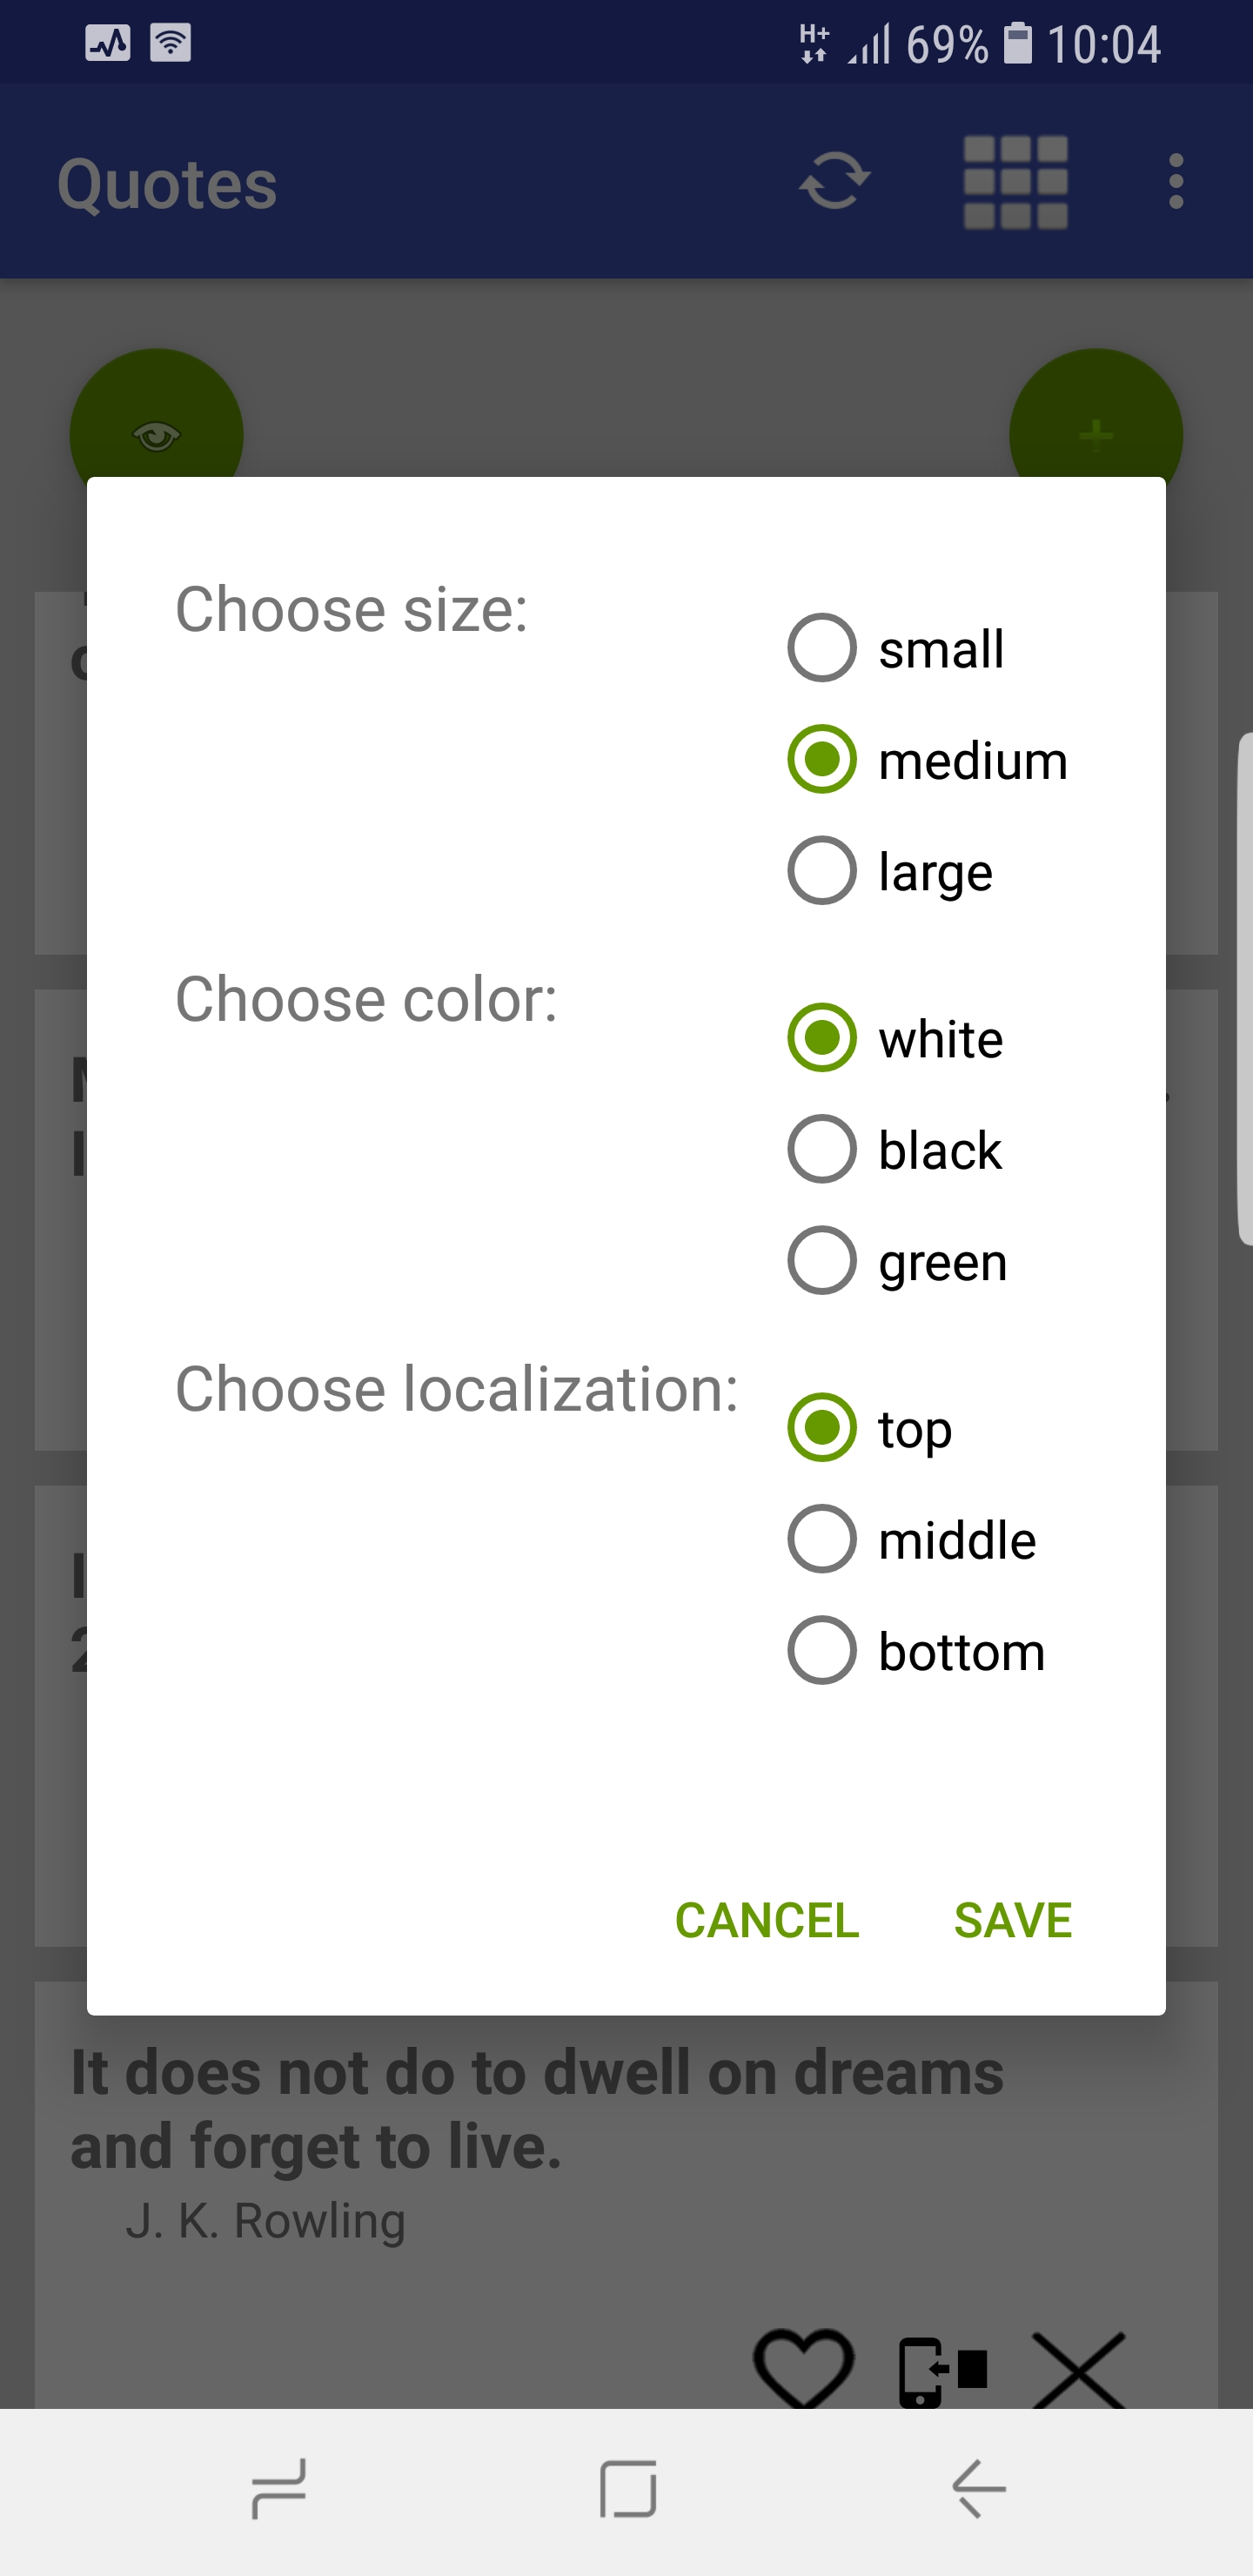
\includegraphics[width=.5\linewidth]{imgs/TuneQuote.jpg}
  \caption{Possibility to tune quote parameters}
  \label{fig:sub1}
\end{subfigure}%
\begin{subfigure}{.55\textwidth}
  \centering
  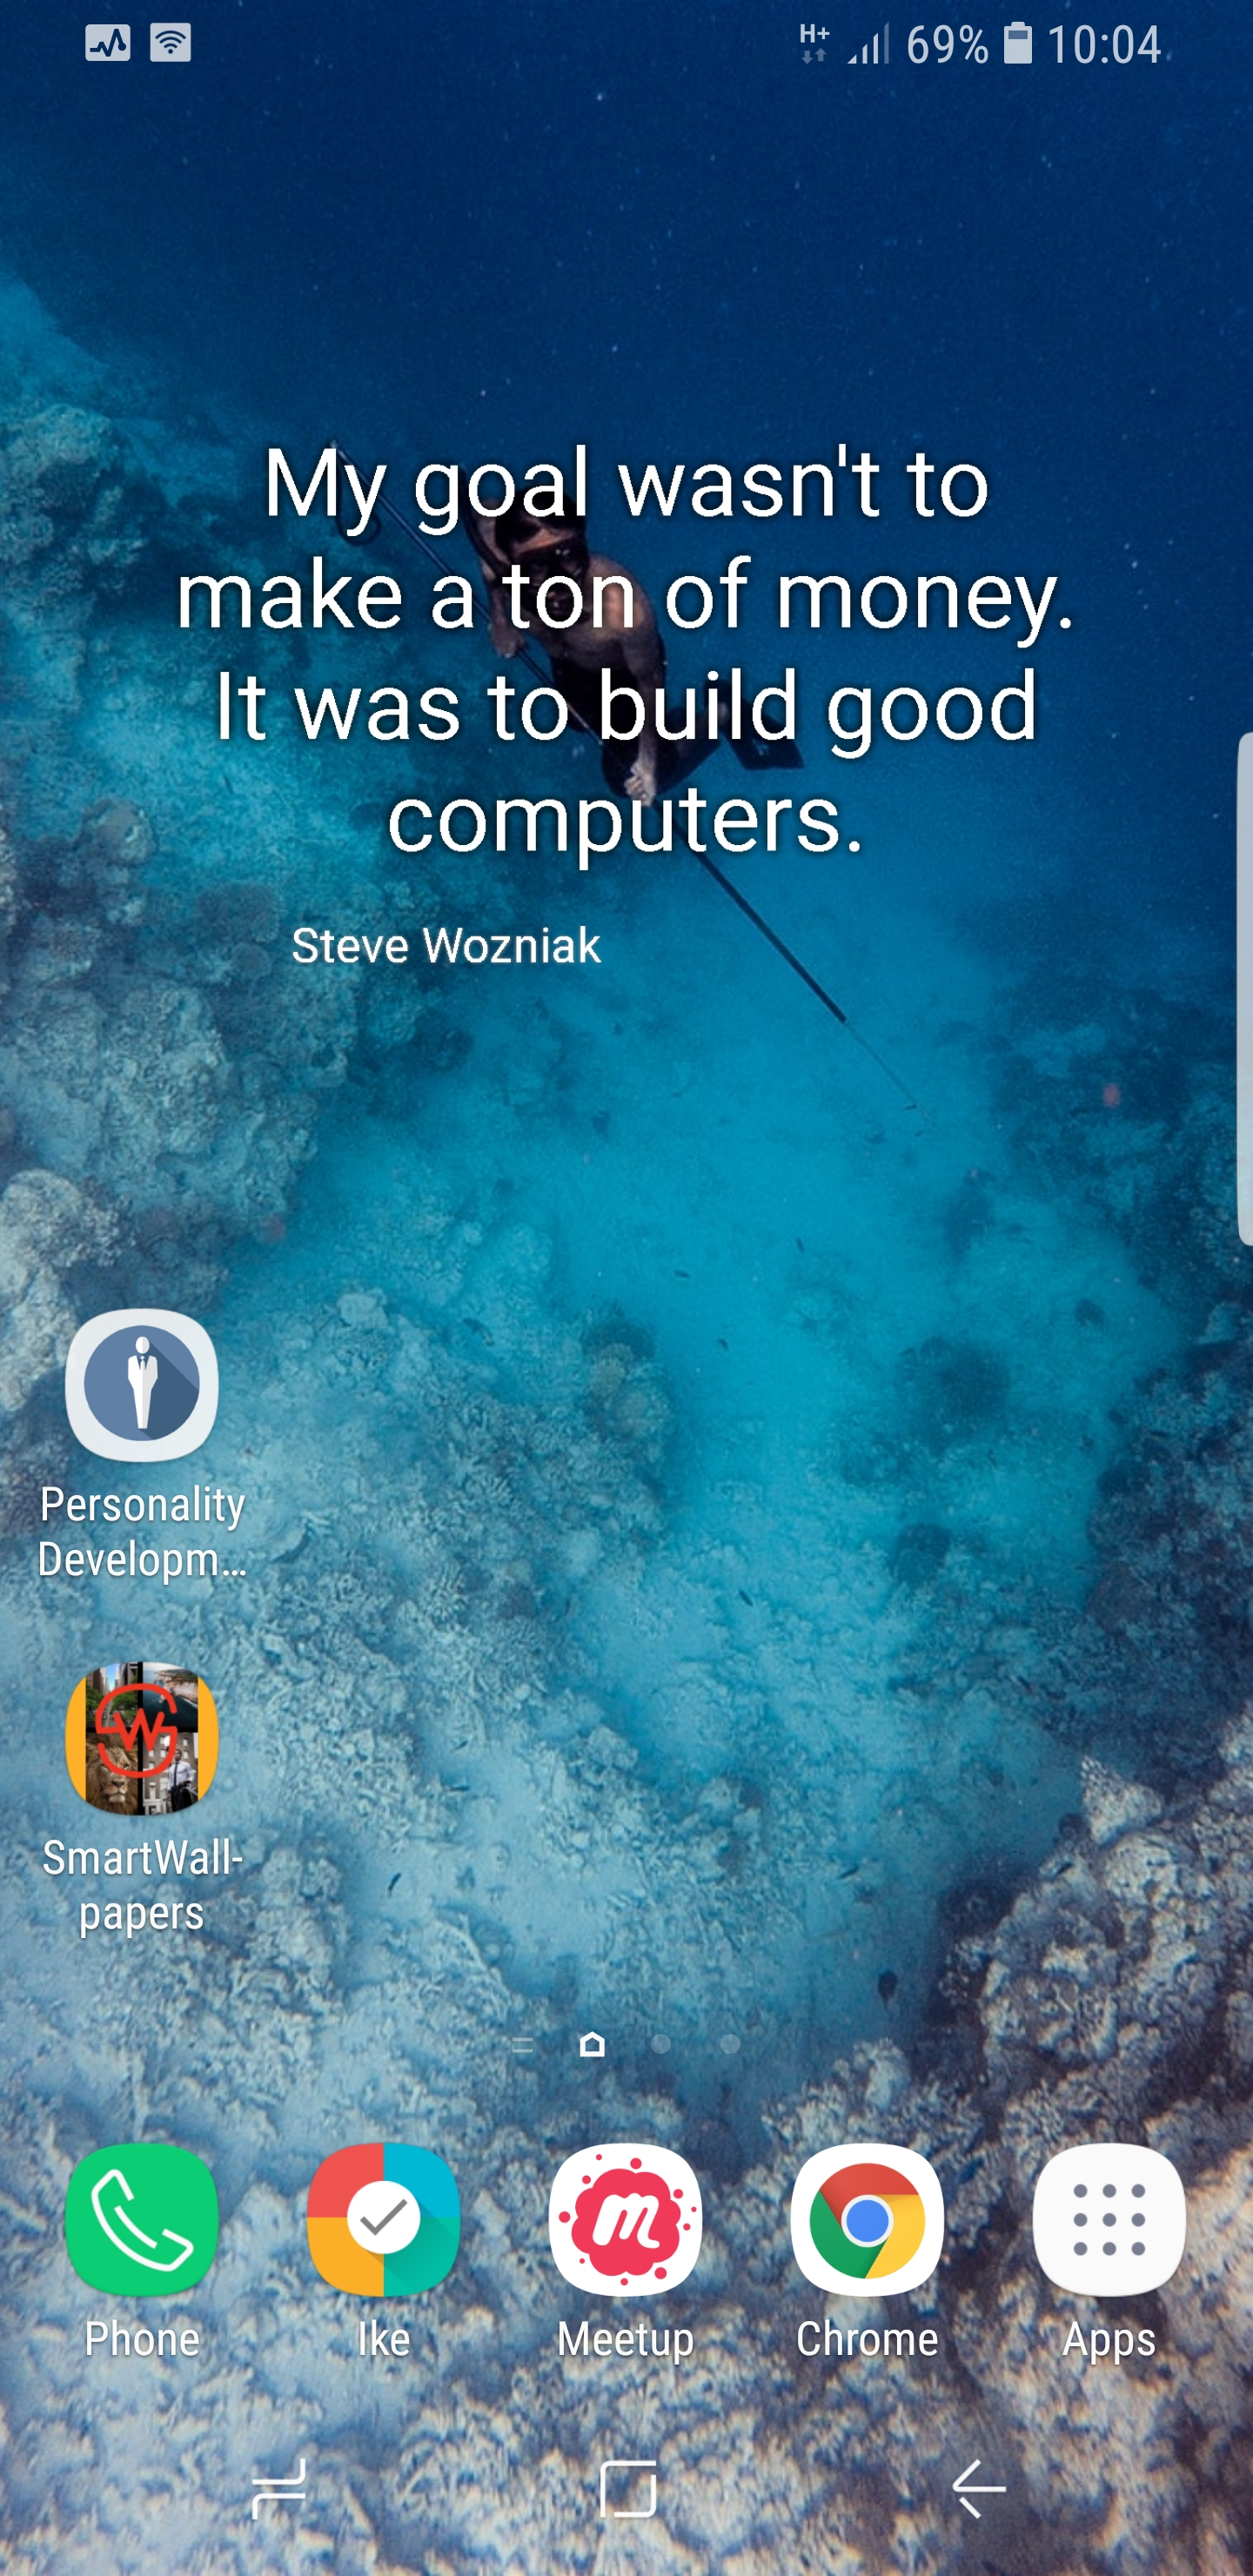
\includegraphics[width=.5\linewidth]{imgs/QuoteHomeScreen.jpg}
  \caption{Quote displayed on the home-screen according to user's selected configuration}
  \label{fig:sub2}
\end{subfigure}
\caption{Interacting with a quote in order to display it on the home-screen}
\label{fig:setQuote}
\end{figure}

\subsection{Add quote by user interface}
	To add a new quote the user should use the top-right button ( "+" icon) and to see the quotes added by him should use the top-left button (eye icon) from quotes main screen (see Figure~\ref{fig:quotes}). After the user inputs the quote he/she wants to add there are three possible actions: cancel, save and like. The functionality of cancel and save buttons is obvious, the like button will save and also set the quote on the home-screen. Notice how the colours of the buttons are chosen in this screen. 	

\begin{figure}[H]
\centering
\begin{subfigure}{.55\textwidth}
  \centering
  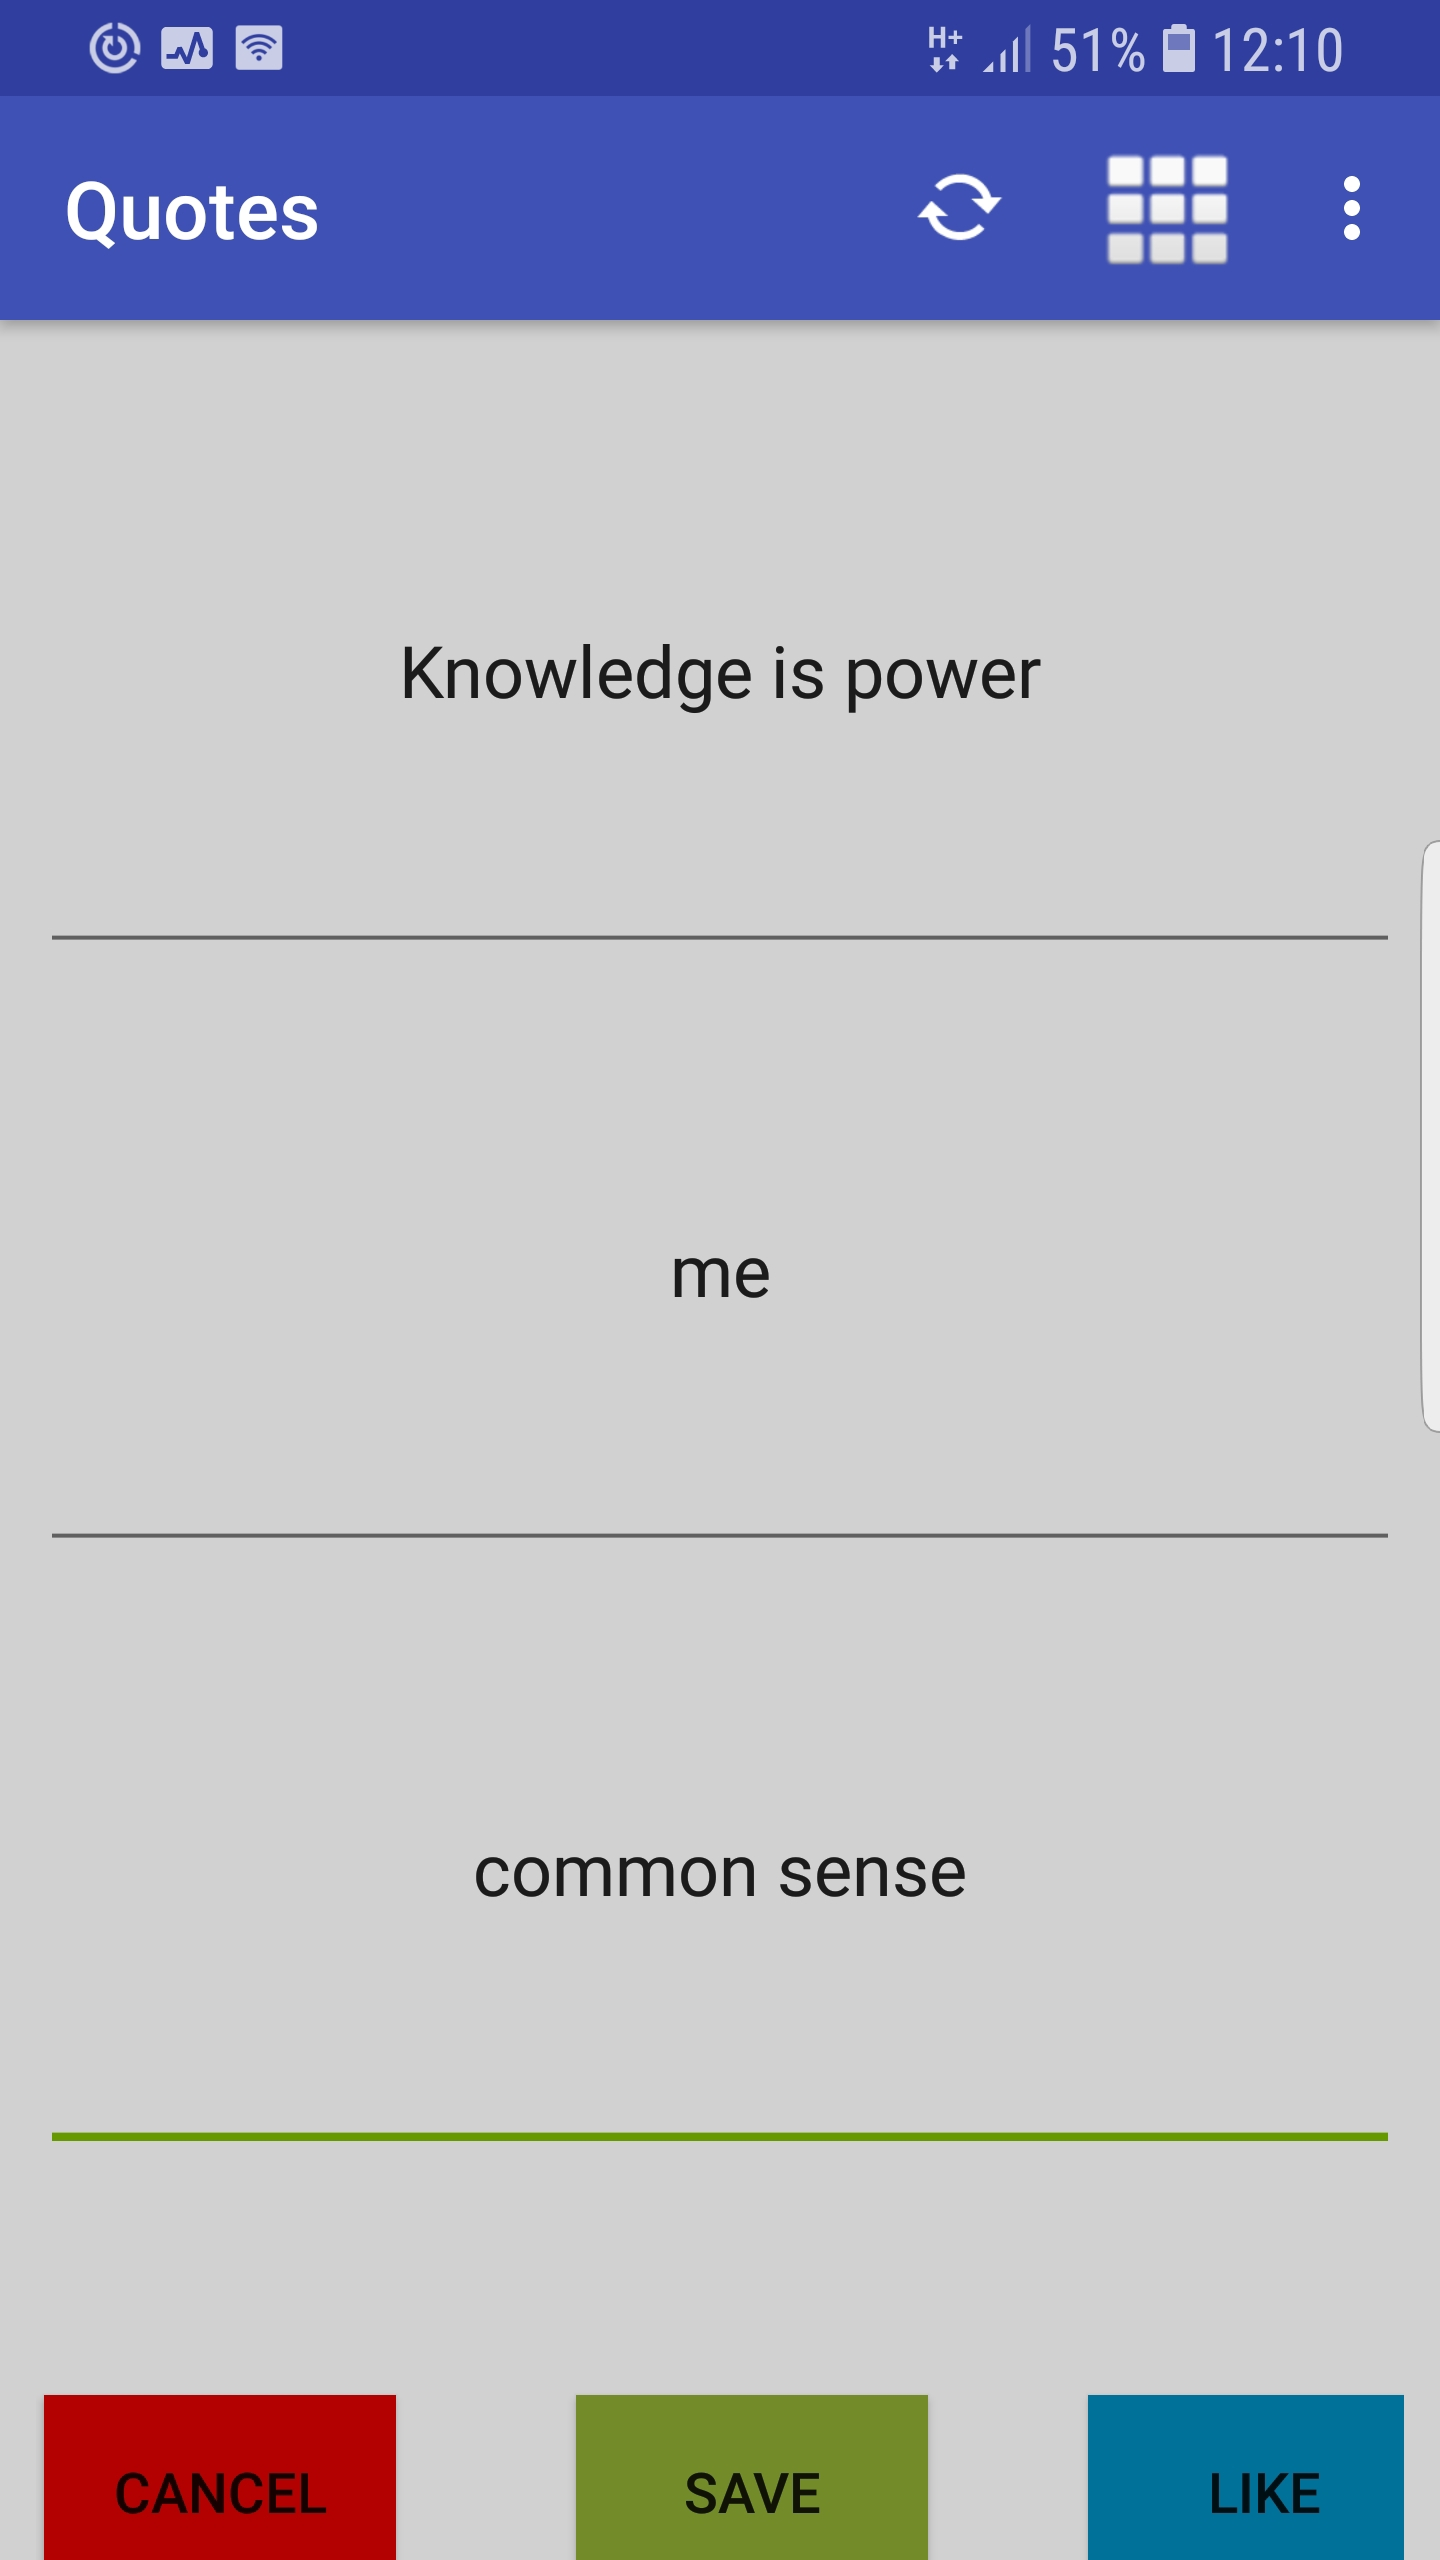
\includegraphics[width=.5\linewidth]{imgs/AddQuote.jpg}
  \caption{View for adding a new quote by user}
  \label{fig:subAddQ}
\end{subfigure}%
\begin{subfigure}{.55\textwidth}
  \centering
  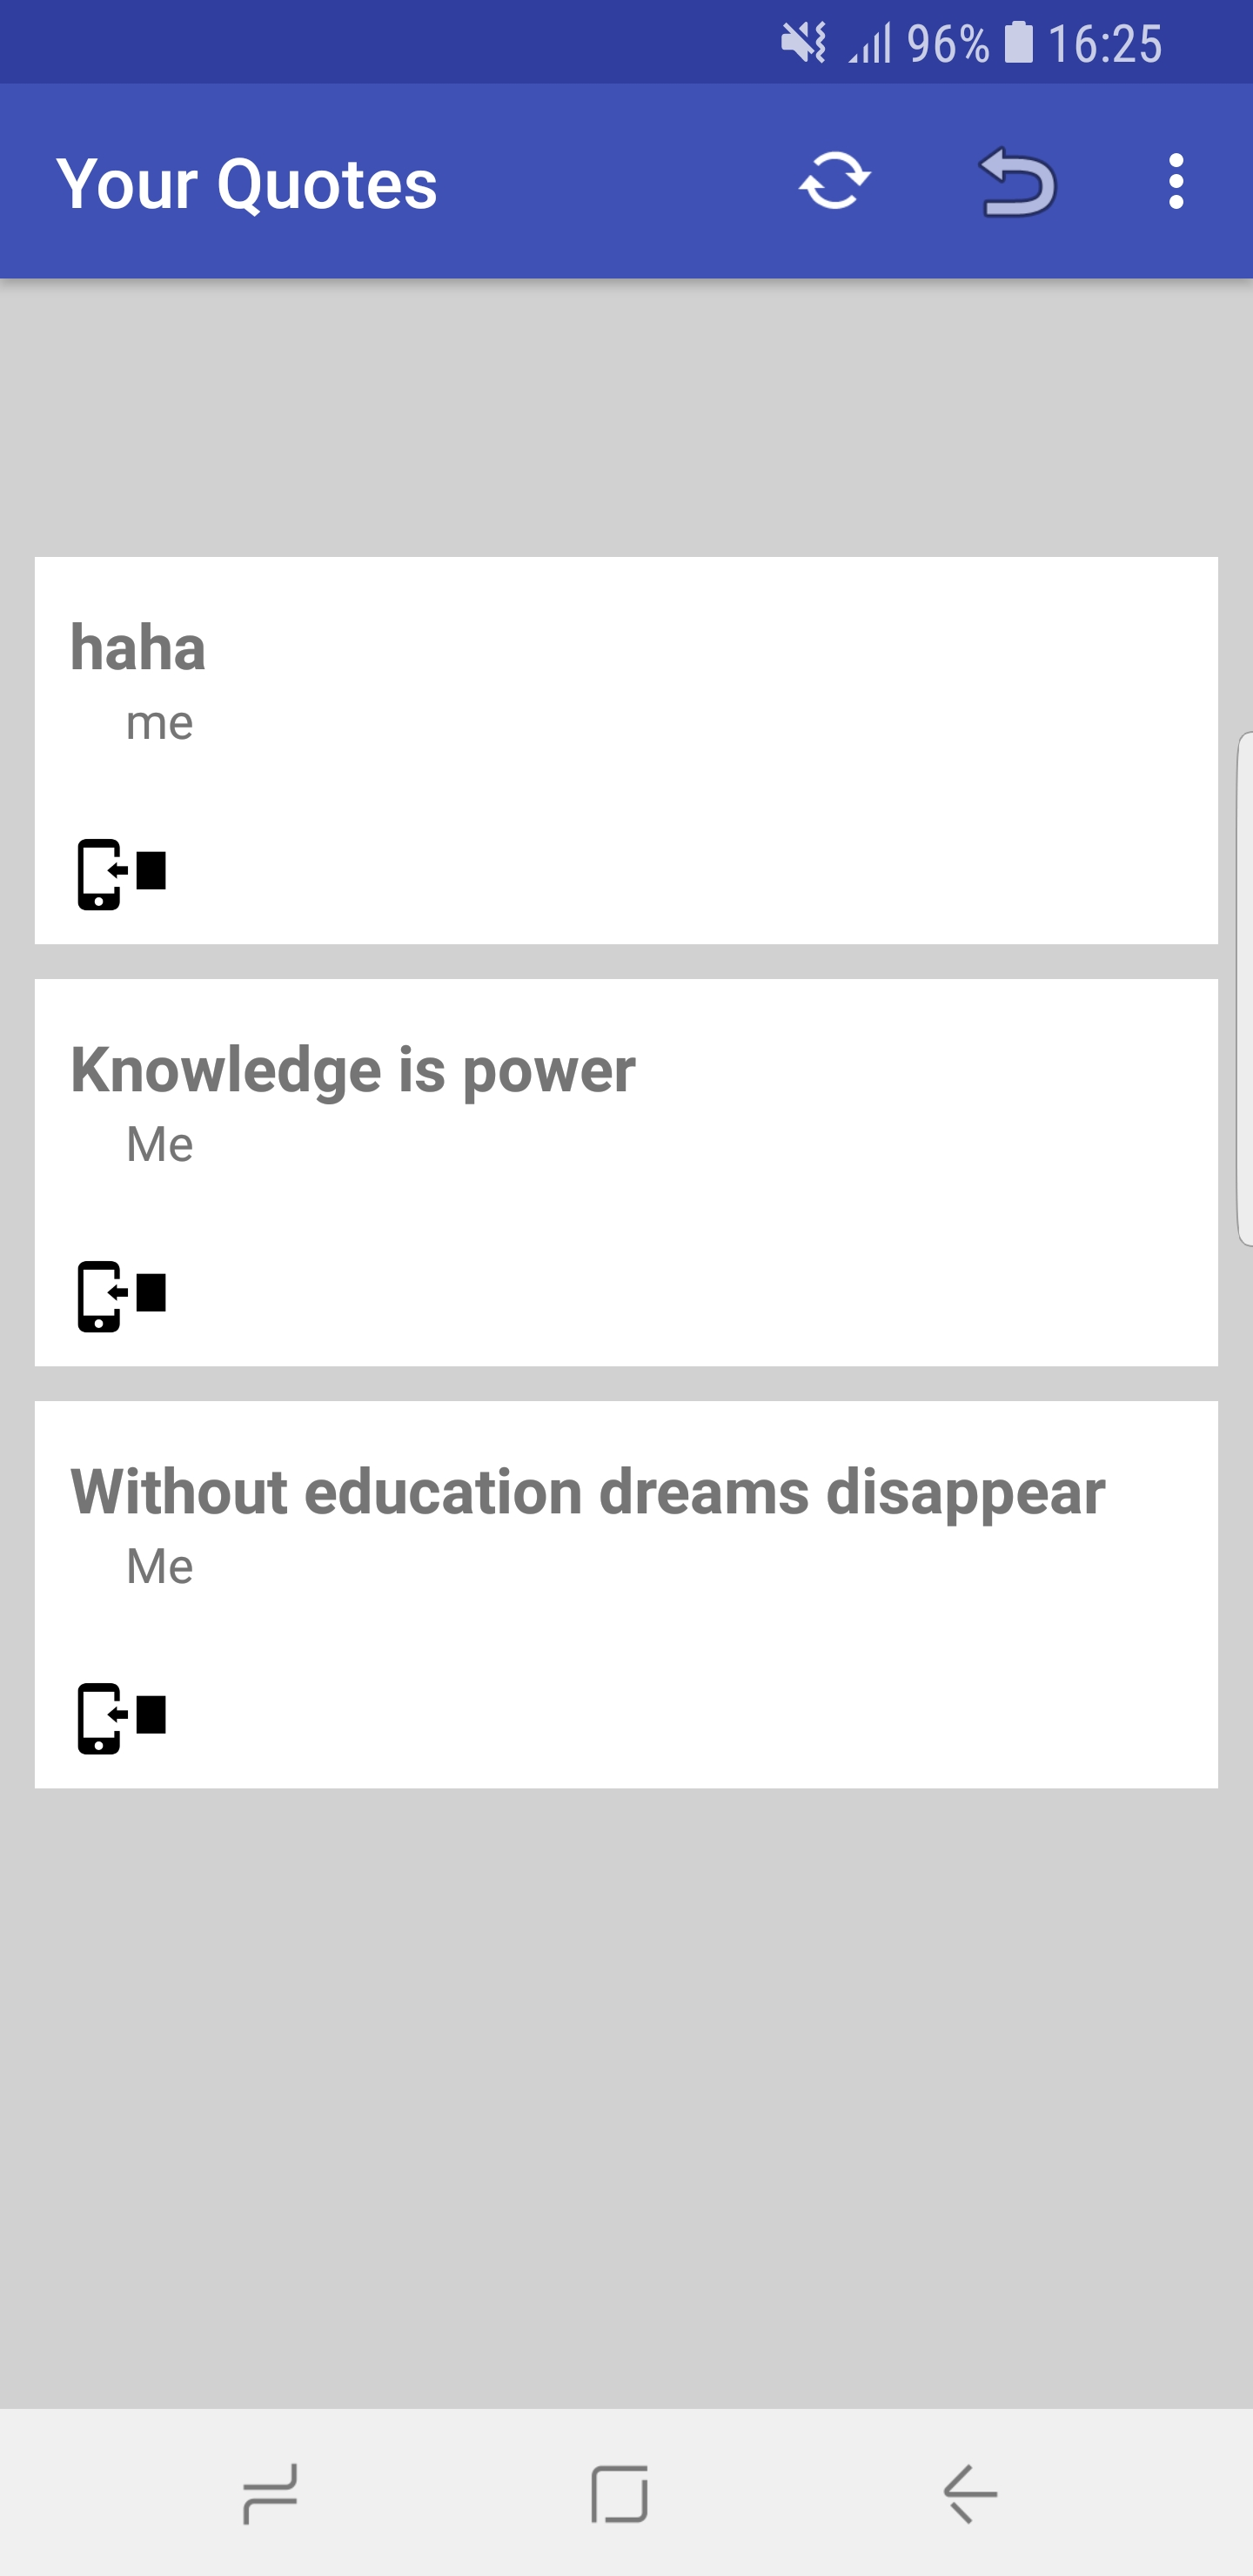
\includegraphics[width=.5\linewidth]{imgs/My_Quotes.jpg}
  \caption{View showing quotes added by the user}
  \label{fig:sub2}
\end{subfigure}
\caption{User's favourite quotes}
\label{fig:usersQuotes}
\end{figure}

\subsection{Accessing other features interface}
	 SmartWallpapers prototype app provides several other screens and interactions. It contains a brief tutorial on how to use the app, the possibility to see what type of photography the user likes the most according to SmartWallpaper analysis of the liked photos, the screen to set the wallpaper-change interval and a screen to provide feedback to developers. 

\begin{figure}[H]
	
	\centering
	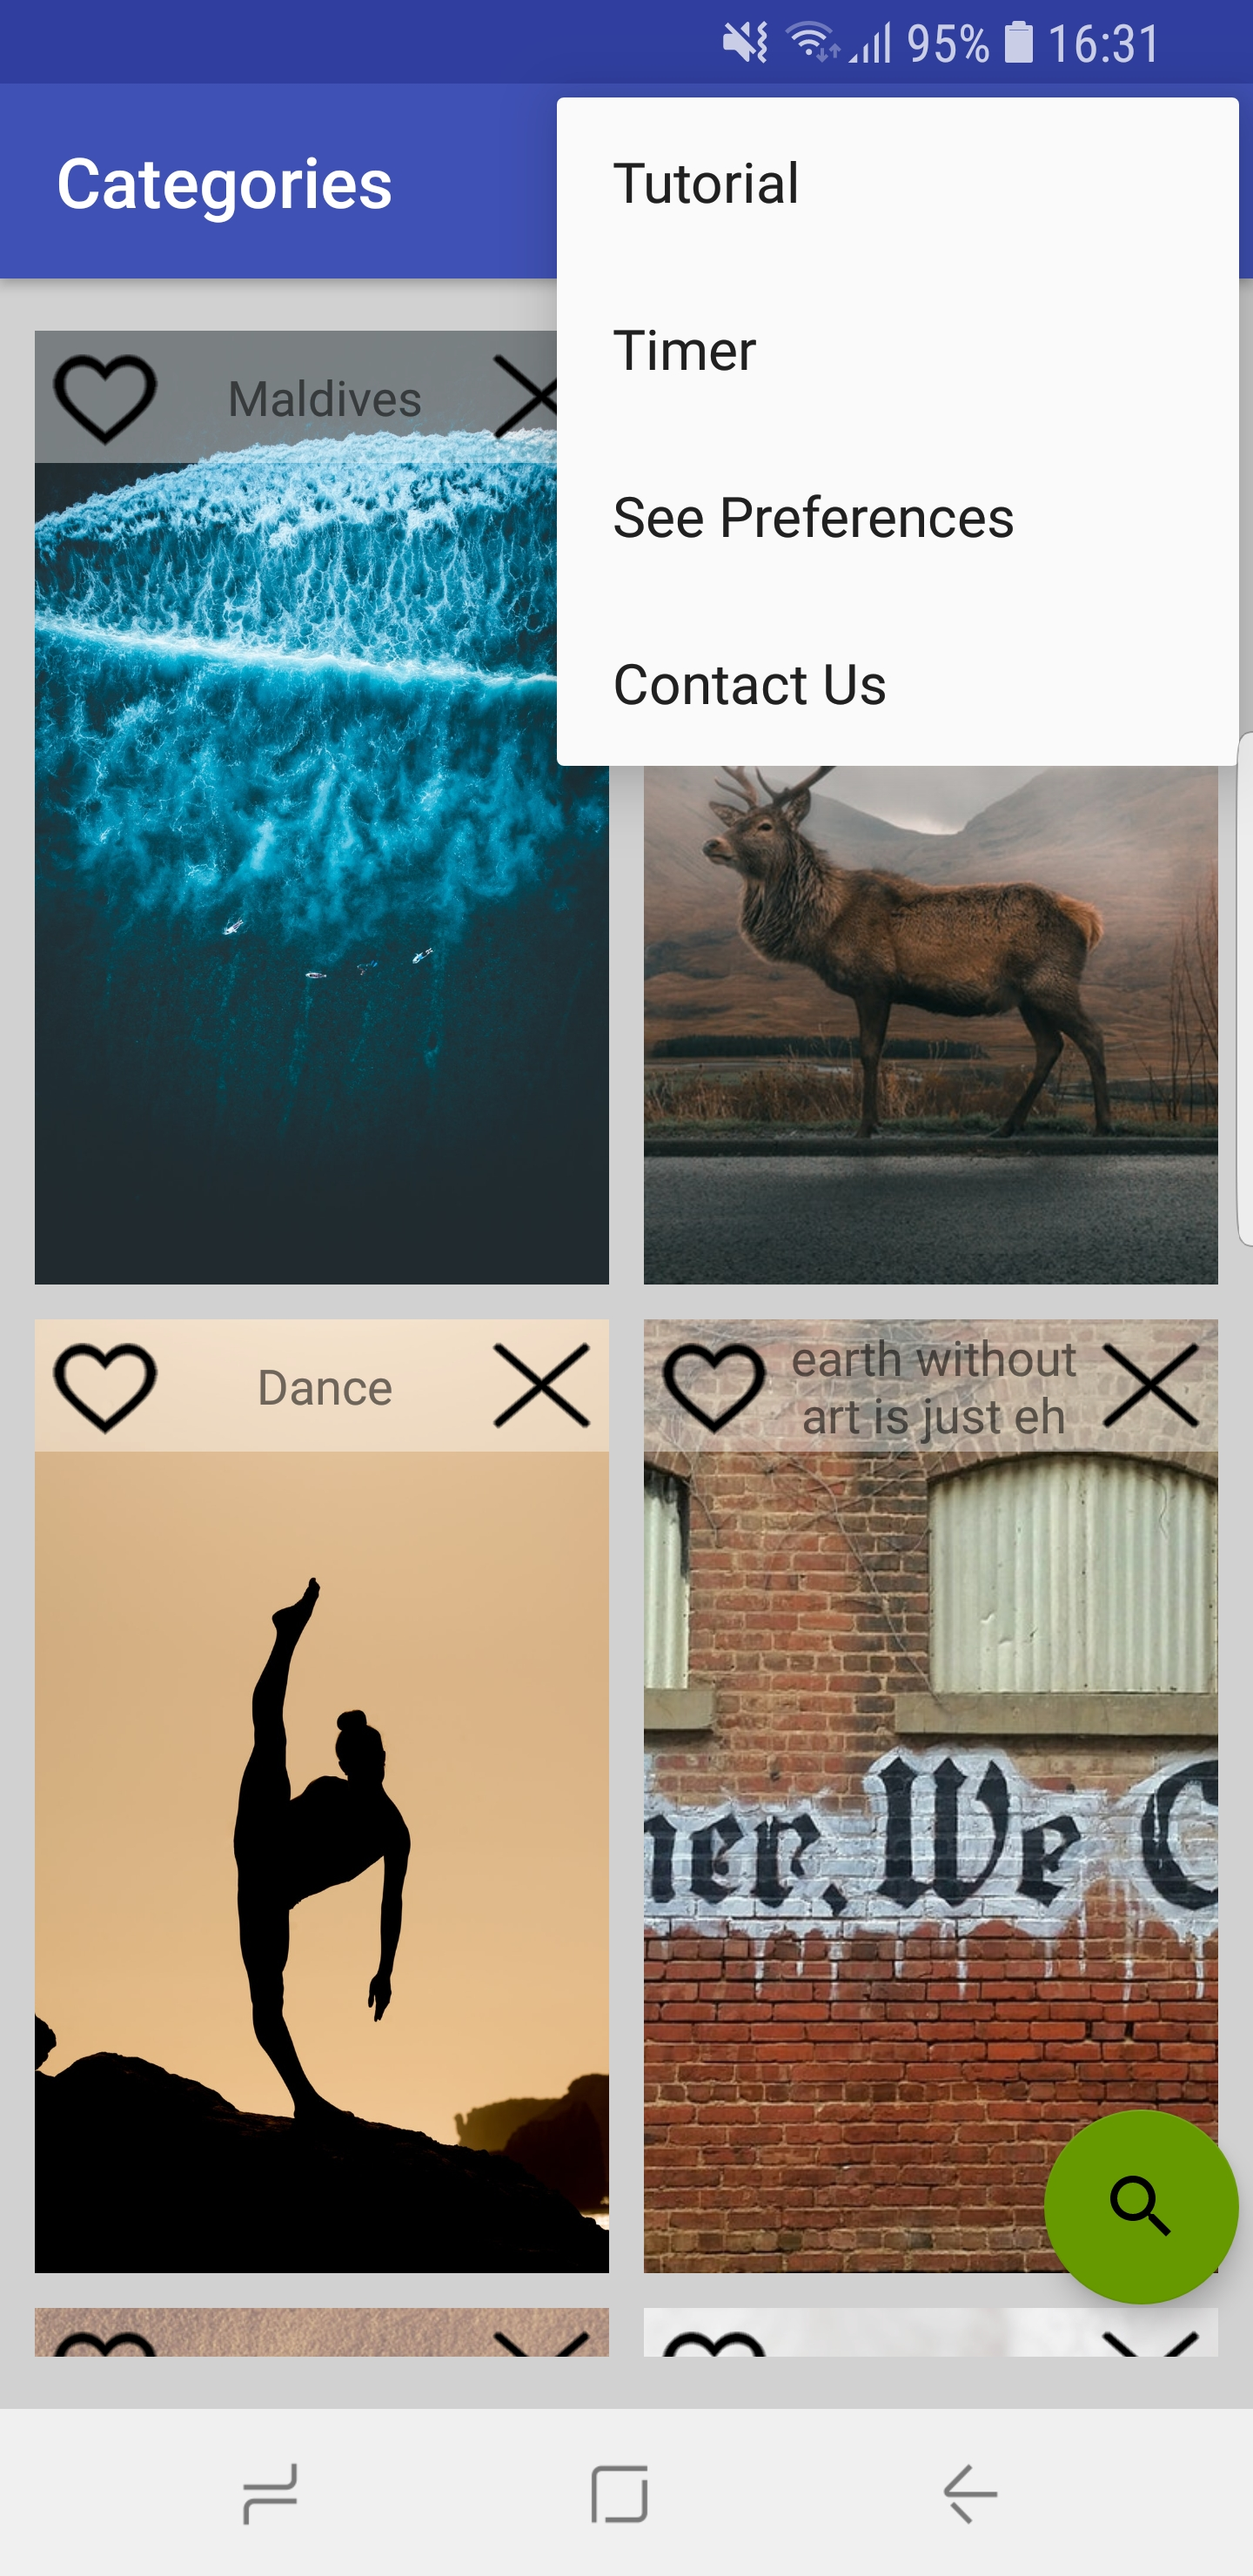
\includegraphics[width = 0.3\textwidth]{imgs/Options.jpg}
	\caption*{Other types of interactions in SmartWallpaper prototype app}

\end{figure}

\section{Evaluation}
	 In order to evaluate each interaction the author is going to do a cognitive walkthrough for each one of them.

\subsection{Photo categories interface}

\subsection{Contents of category interface}

\subsection{Search feature interface}

\subsection{Quotes feature interface}

\subsection{Add quote by user interface}

\subsection{Accessing other features interface}

\section{Conclusions}

\section{Presentation}

\section{References}
Apple. (2018) Available: https://developer.apple.com/design/human-interface-guidelines/ios/overview/themes/ [Accessed: 10 December 2018].\\

Google. (2018) Available: https://developer.android.com/design/ [Accessed: 10 December 2018]. \\

Norman, D. (2013) The Design Of Everyday Things, Revised And Expanded Edition. New York: Basic Books.\\
\end{document}

